\chapter{Abstract Vector Spaces}
\label{chap:abstract-vector-spaces}

The geometric interpretation of vectors developed in the
\hyperref[chap:linear-geometry]{previous chapter} leaves a lot of tones unsung.
We \hyperref[def:space]{defined} the space the vectors occupy as $\R^{n}$. This
definition works well for building intuition but can't get us very far in the
theory of linear systems. You see, the solution sets to linear systems are
rarely equal to $\R^{n}$ for any $n$. But they \emph{are}, in a very literal
sense, `spaces of vectors'.

To illustrate what we mean, consider again the linear equation
\[
 x - y + z = 4
\]
from \myref{section}{sec:visualisation-of-linear-systems-revisited}. Its
solution set is the set of vectors
\[
 \left\{ 
  \begin{pmatrix}
   4\\
   0\\
   0
  \end{pmatrix} + y
  \begin{pmatrix}
   1\\
   1\\
   0
  \end{pmatrix} + z
  \begin{pmatrix}
   -1\\
   0\\
   1
  \end{pmatrix} \mid y,z \in \R
 \right\}.
\]
The vector $\begin{psmallmatrix} 4\\0\\0 \end{psmallmatrix}$ is just a single
shift but the set
\[
 S \coloneqq \left\{ 
  y\begin{pmatrix}
   1\\
   1\\
   0
  \end{pmatrix} + z
  \begin{pmatrix}
   -1\\
   0\\
   1
  \end{pmatrix} \mid y,z \in \R
 \right\}
\]
indeed is an entire `space' of vectors, in the sense that it behaves essentially
the same as $\R^2$. To highlight certain qualities:
\begin{itemize}
 \item It's a plane in $\R^3$; a two-dimensional object, just like $\R^2$ is a
  two-dimensional space.
 \item It contains the origin -- the vector $\begin{psmallmatrix} 0\\0\\0
  \end{psmallmatrix}$.
 \item Adding vectors in $S$ gives a vector in $S$. We cannot ever leave the
  plane just by moving along the vectors in the same plane.
 \item Multiplying vectors from $S$ by real numbers also gives a vector in $S$.
  Enlarging or shortening a vector also doesn't allow us to leave the plane.
\end{itemize}
In this chapter, we shall endeavour to formalize the just outlined concept of a
`set of vectors which behaves just like a space does'. We're going to call these
spaces \emph{abstract vector spaces} or just \emph{vector spaces} for short.

The most important idea behind the definition of a vector space (or a space in
general) is `closedness'. A space ought to be a universe in itself, interactions
between elements cannot ever lead to the creation of an element which is not
present. Mathematicians tend to call these interactions, \emph{operations}, and
label sets which meet this criterion as \emph{closed}. There are a few other
formal requirements we must enforce (e.g. commutativity and associativity of
operations which we take for granted in the real numbers) but the primary aim
remains to define a \emph{closed} set, a space moving along whose vectors allows
one not to escape it.

We thus proceed to define an abstract vector space as a set of vectors which can
be added together and scaled by real numbers by listing axioms (basically
enforced rules of behaviour) the set must satisfy.

\begin{definition}{Abstract vector space}{abstract-vector-space}
 An \emph{(abstract) vector space} over $\R$ is a set $V$ (whose elements style
 \emph{vectors}) together with operations $ \oplus :V \times V \to V$ (called
 \emph{vector addition}) and $\odot: \R \times V \to V$ (called \emph{scalar
 multiplication}) satisfying the following axioms.
 \begin{enumerate}
  \item The operation $ \oplus $ is \emph{commutative}, i.e. $\mathbf{v} \oplus
   \mathbf{w} = \mathbf{w} \oplus \mathbf{v}$ for every
   $\mathbf{v},\mathbf{w} \in V$.
  \item The operation $ \oplus $ is \emph{associative}, i.e. $\mathbf{u} \oplus
   (\mathbf{v} \oplus \mathbf{w}) = (\mathbf{u} \oplus \mathbf{v}) \oplus
   \mathbf{w}$ for every $\mathbf{u},\mathbf{v},\mathbf{w} \in V$.
  \item The set $V$ is \emph{closed} under the operation $ \oplus $, i.e.
   $\mathbf{v} \oplus \mathbf{w} \in V$ whenever $\mathbf{v},\mathbf{w} \in V$.
  \item There exists a \emph{zero vector}, i.e. a vector $\mathbf{0} \in V$ such
   that $\mathbf{v} + \mathbf{0} = \mathbf{v}$ for every $\mathbf{v} \in V$.
  \item Each vector $\mathbf{v} \in V$ has an \emph{additive inverse}, i.e. a
   vector $\mathbf{w} \in V$ such that $\mathbf{v} + \mathbf{w} = \mathbf{0}$.
  \item The operation $\odot$ distributes over $+$, that is, $(r + s) \odot
   \mathbf{v} = r \odot \mathbf{v} \oplus s \odot \mathbf{v}$ for all $r,s \in
   \R$ and $\mathbf{v} \in V$.
  \item The operation $\odot$ distributes over $ \oplus $, i.e. $r \odot
   (\mathbf{v} \oplus \mathbf{w}) = r \odot \mathbf{v} \oplus r \odot
   \mathbf{w}$ for every $r \in \R$ and $\mathbf{v},\mathbf{w} \in V$.
  \item Ordinary multiplication (of real numbers) associates with $\odot$, i.e.
   $(rs) \odot \mathbf{v} = r \odot (s \odot \mathbf{v})$ for every $r,s \in \R$
   and $\mathbf{v} \in V$.
  \item The set $V$ is \emph{closed} under $\odot$, that is, $r \odot
   \mathbf{v} \in V$ whenever $r \in \R$ and $\mathbf{v} \in V$.
  \item Scalar multiplication by $1$ acts as the \emph{identity operation}, that
   is, $1\odot \mathbf{v} = \mathbf{v}$ for every $\mathbf{v} \in V$.
 \end{enumerate}
\end{definition}

\begin{figure}[ht]
 \centering
 \begin{subfigure}[c]{.45\textwidth}
  \centering
  \begin{tikzpicture}
   \tkzDefPoints{0/0/O,1/3/a,3/1/b,4/4/c}
   \tkzDrawSegment[-Latex,thick,BrickRed](O,a)
   \tkzDrawSegment[-Latex,thick,RoyalBlue](a,c)
   \tkzDrawSegment[-Latex,thick,RoyalBlue](O,b)
   \tkzDrawSegment[-Latex,thick,BrickRed](b,c)
   \tkzDrawSegment[-Latex,thick,dashed,ForestGreen](O,c)
   \tkzLabelSegment[BrickRed,left=1mm](O,a){$\mathbf{v}$}
   \tkzLabelSegment[BrickRed,right=1mm](b,c){$\mathbf{v}$}
   \tkzLabelSegment[RoyalBlue,above=1mm](a,c){$\mathbf{w}$}
   \tkzLabelSegment[RoyalBlue,below=1mm](O,b){$\mathbf{w}$}
   \tkzLabelSegment[ForestGreen,above left](O,c){$\mathbf{v} + \mathbf{w}$}
   \tkzLabelSegment[ForestGreen,below right](O,c){$\mathbf{w} + \mathbf{v}$}
  \end{tikzpicture}
 \end{subfigure}
 \begin{subfigure}[c]{.45\textwidth}
  \centering
  \begin{tikzpicture}[scale=0.9]
   \tkzDefPoints{0/0/O,2/2/a,5/2/b,7/0/c}
   \tkzDrawSegment[-Latex,thick,BrickRed](O,a)
   \tkzDrawSegment[-Latex,thick,RoyalBlue](a,b)
   \tkzDrawSegment[-Latex,thick,ForestGreen](b,c)
   \tkzLabelSegment[above left,BrickRed](O,a){$\mathbf{u}$}
   \tkzLabelSegment[above=1mm,RoyalBlue](a,b){$\mathbf{v}$}
   \tkzLabelSegment[above right,ForestGreen](b,c){$\mathbf{w}$}
   \tkzDrawSegment[-Latex,thick,dashed](O,b)
   \tkzLabelSegment[above left=1mm and -4mm](O,b){\clr{$\mathbf{u}$} +
   \clb{$\mathbf{v}$}}
   \tkzDrawSegment[-Latex,thick,dashed](a,c)
   \tkzLabelSegment[above right=1mm and -4mm](a,c){\clb{$\mathbf{v}$} +
   \clg{$\mathbf{w}$}}
   \tkzDrawSegment[-Latex,thick,Fuchsia](O,c)
   \tkzLabelSegment[below=1mm](O,c){$(\clr{\mathbf{u}} + \clb{\mathbf{v}}) +
    \clg{\mathbf{w}} = \clr{\mathbf{u}} + (\clb{\mathbf{v}} +
    \clg{\mathbf{w}})$}
  \end{tikzpicture}
 \end{subfigure}
 \caption{The visualization of commutativity and associativity of vector
 addition.}
 \label{fig:vector-addition-com-and-ass}
\end{figure}

\begin{remark}{}{}
 The \hyperref[def:abstract-vector-space]{definition of vector space} hosts a
 plethora of axioms; some for different `mathematical' reasons than others.

 The axioms (3) and (9) are the `most important' in a sense. They ascertain that
 the resulting set is indeed a space, in the sense discussed in the introduction
 to \hyperref[chap:abstract-vector-spaces]{this chapter}.

 The axioms (1), (2), (6), (7), (8) and (10) are technical. Their role is to
 make vectors and numbers interact in a way we find intuitive hailing from
 $n$-dimensional real spaces. There, we take for granted the sum of two vectors
 is invariant under change of the order of summation but, on the other hand, one
 can easily design sets of elements with an addition operation not commutative.
 The gist of it is that we still wish to think of elements of vector spaces as
 \dots~well \dots~vectors, and once a vector, you should behave like a vector.

 Finally, axioms (4) and (5) are there so that we can `reverse arrows', in a
 sense. Again, we tend to treat vectors as measures of length and direction so
 it makes sense to be able to travel the same distance in a direction opposite.
 The condition of being able to reverse brings with it the necessity to have an
 `original point' since otherwise the sum of a vector with its additive inverse
 would send us flying out of the space we're in. That ought not to happen.
\end{remark}

\begin{remark}{}{}
 Diligent readers have surely noticed that we denoted the operations $ \oplus $
 and $\odot$ on an \hyperref[def:abstract-vector-space]{abstract vector space}
 differently than we would before. For predominantly didactic reasons. When we
 first defined \hyperref[def:adding-vectors]{vector addition}, we didn't feel
 the need to distinguish adding two real numbers from adding two vectors because
 vector addition is just component-wise addition of numbers anyway. However,
 elements of an abstract vector space can (as we shall soon see) actually be
 somewhat distant from the intuitive image of vectors we harbour. It seemed apt
 to fully convey the perception of difference between vector addition and
 `normal' addition. Scalar multiplication falls under the same argument.

 Nonetheless, it is common in literature to write the vector addition operation
 $ \oplus $ the same way as the addition of real numbers and we purport to
 adhere to the norm. However, we shall at least make the distinction between
 scalar multiplication and real multiplication by using the symbol $ \cdot $ for
 the former and lack of a symbol for the latter. The operation $ \cdot $ of
 scalar multiplication ought not to be confused with
 \hyperref[def:dot-product]{dot product} which we have not defined for abstract
 vectors.
\end{remark}

We fare ahead and list quite a few examples of
\hyperref[def:abstract-vector-space]{abstract vector spaces}. Some should come
as no surprise, some as quite it.

\begin{example}{$n$-dimensional real space}{n-dimensional-real-space}
 An obvious example of a \hyperref[def:abstract-vector-space]{vector space} is
 the $n$-dimensional real space $\R^{n}$. Veracity of the ten axioms is
 trivially checked given that their conception is based on the $\R^{n}$
 archetype.
\end{example}

\begin{example}{Solution sets of homogeneous linear systems}{solution-sets-of-homogeneous-linear-systems}
 The motivating example behind \hyperref[def:abstract-vector-space]{vector
 spaces} have exactly been the sets of vectors like
 \[
  \{r_1 \cdot \mathbf{v}_1 + r_2 \cdot \mathbf{v}_2 + \ldots + r_k \cdot
  \mathbf{v}_k\},
 \]
 which should be `correctly' written as
 \[
  \{r_1 \odot \mathbf{v}_1 \oplus r_2 \odot \mathbf{v}_2 \oplus \ldots \oplus
  r_k \odot \mathbf{v}_k\},
 \]
 for some $r_1,\ldots,r_n \in \R$ and $\mathbf{v}_1,\ldots,\mathbf{v}_k \in
 \R^{n}$. These are not \emph{exactly} equal to $\R^{k}$ although they do
 describe a space with $k$ different directions of movement. Since we defined
 vector spaces with the primary aim of accommodating such examples, it would be
 quite the sorry situation should they fail to be them. Luckily, all such sets
 indeed are vector spaces. Naturally, by
 \myref{proposition}{prop:solution-set-of-a-homogeneous-linear-system}, these
 sets arise as sets of solutions of homogeneous linear systems.

 Since they are sets of vectors in $\R^{n}$, the technical axioms (1), (2), (6),
 (7), (8) and (10) are trivially satisfied. We are going to check axioms (3) and
 (9) first. They say that the sum of solutions of a homogeneous linear system is
 also a solution of the same system and so are multiples of solutions. Suppose
 thus that the vectors $\mathbf{v}, \mathbf{w} \in \R^{n}$ are solutions of the
 homogeneous linear system
 \[
  \begin{array}{r c r c c c r c r}
   a_{1,1}x_1 & + & a_{1,2} x_2 & + & \ldots & + & a_{1,n}x_n &= & 0\\
   a_{2,1}x_1 & + & a_{2,2} x_2 & + & \ldots & + & a_{2,n}x_n &= & 0\\
              & & & & & & & \vdots &\\
   a_{m,1}x_1 & + & a_{m,2} x_2 & + & \ldots & + & a_{m,n}x_n &= & 0
  \end{array}
 \]
 Then, for every $i \leq n$, the equality
 \begin{align*}
  a_{i,1}(v_1 + w_1) + a_{i,2}(v_2 + w_2) + \ldots + a_{i,n}(v_n + w_n) &=
  a_{i,1}v_1 + a_{i,2}v_2 + \ldots + a_{i,n}v_n \\
                                                                        &+
  a_{i,1}w_1 + a_{i,2}w_2 + \ldots + a_{i,n}w_n\\
                                                                        &=
  0 + 0 = 0
 \end{align*}
 is satisfied, which proves (3). Similarly, if $\mathbf{v}$ is a solution, then
 for any $r \in \R$ and all $i \leq n$ we have
 \begin{align*}
  a_{i,1}(rv_1) + a_{i,2}(rv_2) + \ldots + a_{i,n}(rv_n) &= ra_{i,1}v_1 +
  ra_{i,2}v_2 + \ldots + ra_{i,n}v_n\\
                                                         &= r(a_{i,1}v_1 +
                                                         a_{i,2}v_2 + \ldots +
                                                         a_{i,n}v_n) = 0,
 \end{align*}
 which means that $r \cdot \mathbf{v}$ is also a solution, and thus (9) holds.

 Finally, as far as axioms (4) and (5) are concerned, the vector $\mathbf{0}$ is
 always a solution of a homogeneous linear system and the inverse to a solution
 $\mathbf{v}$ is, of course, the solution $-1 \cdot \mathbf{v}$ (which is indeed
 a solution by the preceding paragraph).
\end{example}

\begin{remark}{}{linear-systems-not-spaces}
 Do note that by
 \myref{example}{exam:solution-sets-of-homogeneous-linear-systems}, only the
 solutions of \textbf{homogeneous} linear systems are vector spaces. Solutions
 to non-homogeneous linear systems \textbf{always} fail to be vector spaces;
 they do not contain the vector $\mathbf{0}$ for example. They are so-called
 \emph{affine} spaces which we shan't study in this text.
\end{remark}

\begin{example}{Sets of polynomials}{sets-of-polynomials}
 Sets of polynomials in one variable of a given degree make an interesting
 example of an \hyperref[def:abstract-vector-space]{abstract vector space}. To
 recall, a real polynomial $p$ in one variable of degree $n$ is the expression
 \[
  p(x) = r_0 + r_1x + r_2x^2 + \ldots + r_n x^{n}
 \]
 for some $r_0,\ldots,r_n \in \R$. We claim that the set
 \[
  \{p \mid p \text{ is a real polynomial of degree } n\},
 \]
 with the addition operation being the typical addition of polynomials and
 scalar multiplication being simple multiplication of polynomials by real
 numbers, is a vector space.

 Similarly to the
 \hyperref[exam:solution-sets-of-homogeneous-linear-systems]{previous example},
 axioms (1), (2), (6), (7), (8) and (10) are easily verified to hold. Clearly,
 the sum of two polynomials of degree $n$ is a polynomial of degree $n$ and the
 multiple of a polynomial of degree $n$ is again a polynomial degree $n$. The
 zero vector is the polynomial $0 + 0x + 0x^2 + \ldots + 0x^{n}$ and the inverse
 to the polynomial $p$ is of course $-p$.

 Do note however that we \textbf{forbid polynomial multiplication} since the
 product of two polynomials of degree $n$ is no longer a polynomial of degree
 $n$. We may only add polynomials and multiply them by a real number.

 As a matter of fact, polynomials of degree $n$ are in a sense `the same' as
 vectors over $\R^{n+1}$. The correspondence is easy to forge -- we simply
 encode the coefficients of the polynomial into a vector like so:
 \[
  r_0 + r_1x + r_2x^2 + \ldots + r_nx^{n} \mapsto 
  \begin{pmatrix}
   r_0\\
   r_1\\
   r_2\\
   \vdots\\
   r_n
  \end{pmatrix} \in \R^{n+1}.
 \]
 We can now rewrite polynomial addition and scalar multiplication as the same
 operations on vectors in $\R^{n+1}$. For example, on the set of polynomials of
 degree $3$, the addition
 \[
  (2x + x^2 + 3x^3) + (-1 + 3x - 5x^3) = -1 + 5x + x^2 - 2x^3
 \]
 can be written in the following vector form.
 \[
  \begin{pmatrix}
   0\\
   2\\
   1\\
   3
  \end{pmatrix}
  + 
  \begin{pmatrix}
   -1\\
   3\\
   0\\
   -5
  \end{pmatrix}
  = 
  \begin{pmatrix}
   -1\\
   5\\
   1\\
   -2
  \end{pmatrix}
 \]
\end{example}

\begin{example}{Matrices}{matrices}
 The set
 \[
  \left\{
   \begin{pmatrix}
    a_{11} & a_{12}\\
    a_{21} & a_{22}
   \end{pmatrix}
   \mid a_{11},a_{12},a_{21},a_{22} \in \R
  \right\}
 \]
 of $2 \times 2$ matrices with real entries and entry-wise addition and
 scalar multiplication is a \hyperref[def:abstract-vector-space]{vector space}
 over $\R$. This space is often denoted as $\R^{2 \times 2}$. To give an
 example, the addition of matrices behaves like this:
 \[
  \begin{pmatrix}
   1 & 2\\
   3 & 4
  \end{pmatrix}
  + 
  \begin{pmatrix}
   2 & 1\\
   4 & 3\\
  \end{pmatrix}
  = 
  \begin{pmatrix}
   1 + 2 & 2 + 1\\
   3 + 4 & 4 + 3
  \end{pmatrix}
  =
  \begin{pmatrix}
   3 & 3\\
   7 & 7
  \end{pmatrix};
 \]
 and scalar multiplication like this:
 \[
  2 \cdot 
  \begin{pmatrix}
   1 & 2\\
   3 & 4
  \end{pmatrix}
  =
  \begin{pmatrix}
   2 \cdot 1 & 2 \cdot 2\\
   2 \cdot 3 & 2 \cdot 4
  \end{pmatrix}
  = 
  \begin{pmatrix}
   2 & 4\\
   6 & 8
  \end{pmatrix}.
 \]
 Upon closer inspection, $2 \times 2$ matrices behave exactly like $4$-component
 real vectors. Indeed, we can find a correspondence
 \[
  \begin{pmatrix}
   a_{11} & a_{12}\\
   a_{21} & a_{22}
  \end{pmatrix}
  \longleftrightarrow
  \begin{pmatrix}
   a_{11}\\
   a_{12}\\
   a_{21}\\
   a_{22}
  \end{pmatrix}
 \]
 and treat the space $\R^{2 \times 2}$ exactly the same as $\R^{4}$ with vector
 addition and multiplication. This correspondence also shows that all the
 defining axioms are satisfied.

 This example can naturally be scaled to spaces $\R^{m \times n}$ of real
 matrices with $m$ rows and $n$ columns. One always gets a correspondence
 between $\R^{m \times n}$ and $\R^{mn}$.
\end{example}

\begin{example}{The trivial space}{the-trivial-space}
 The set $\{\mathbf{0}\}$ containing only the zero vector is a vector space. It
 is actually the smallest (by element count) vector space that can exist. The
 empty set is not a vector space precisely due to its lack of the zero vector.
\end{example}

\begin{example}{Natural functions}{natural-functions}
 The set
 \[
  \{f \mid f \text{ is a function } \N \to \R\},
 \]
 with addition defined by $(f+g)(n) = f(n) + g(n)$ and scalar multiplication by
 $(r \cdot f)(n) = rf(n)$, is a vector space. It differs from previous examples
 by its \emph{dimension}. Without proper means to define the dimension of a
 vector space just yet, we just vaguely state that this vector space has
 \emph{infinite} dimension.

 Each function $f:\N \to \R$ \emph{can} actually be represented as a vector with
 real entries, but with an infinite number of them. For example, the function
 $f(n) = n^2 + 1$ can be represented as a vector
 \[
  \begin{pmatrix}
   f(0)\\
   f(1)\\
   f(2)\\
   \vdots
  \end{pmatrix} = 
  \begin{pmatrix}
   0^2 + 1\\
   1^2 + 1\\
   2^2 + 1\\
   \vdots
  \end{pmatrix}
  =
  \begin{pmatrix}
   1\\
   2\\
   5\\
   \vdots
  \end{pmatrix}
 \]
 whose $i$-th entry is $f(i)$. Since there are infinitely many natural numbers,
 these vectors themselves must have infinite entries. We leave the verification
 of the vector space axioms to our hard-working readers.
\end{example}

\begin{example}{Real functions}{real-functions}
 Our final example features the set of all functions $f:\R \to \R$ with addition
 and scalar multiplication defined as in
 \myref{example}{exam:natural-functions}. This is again a vector space
 (exercise) which has not just infinite, but \emph{uncountable} dimension. The
 consequence of this fact is that such functions can no longer be reasonably
 represented as vectors. As real numbers cannot be \emph{enumerated}, we have no
 clear idea what the $i$-th entry of such a vector should be.
\end{example}

\begin{exercise}{}{functions-are-vector-spaces}
 Prove (by checking the axioms) that the sets of functions mentioned in
 examples~\ref{exam:natural-functions} and~\ref{exam:real-functions} are indeed
 vector spaces  \hyperref[def:abstract-vector-space]{by definition}.
\end{exercise}

The string of examples hopefully shed some light on the power of
\emph{abstraction} or \emph{generalisation} in mathematics. It is not that
(most) mathematicians enjoy working with abstract and unintuitive concepts (most
of them refer to them as `abstract nonsense' actually) but that this approach
yields results about many structures at once. Everything we henceforth prove
about vector spaces is going to be valid for all the sets mentioned here as well
as absolutely any set that fits the
\hyperref[def:abstract-vector-space]{definition} of a vector space. To give a
few examples:
\begin{itemize}
 \item the theory of differential equations from calculus relies heavily on the
  description of solutions of linear systems;
 \item multivariable real calculus (differentiation and integration of function
  $f:\R^{m} \to \R^{n}$) uses theory of matrices and their determinants (to be
  introduced way later) as derivatives of multivarible functions are matrices;
 \item vectors and matrices whose entries are module homomorphisms are a regular
  occurrence in my own branch of representation theory of algebras.
\end{itemize}
Had we kept working only in the spaces $\R^{n}$, we would have had to be
constantly doubting whether any one result wasn't particular to this scenario.

We close this introductory passage with some `intuitively obvious' statements
about qualities of vectors that are nevertheless not mentioned as axioms and, as
such, must be proven.

\begin{lemma}{Abstract nonsense}{abstract-nonsense}
 Let $V$ be a vector space over $\R$. Then, for any $r \in \R$ and
 $\mathbf{v} \in V$, we have
 \begin{enumerate}[label=(\alph*)]
  \item $0 \cdot \mathbf{v} = \mathbf{0}$;
  \item $(-1 \cdot \mathbf{v}) + \mathbf{v} = \mathbf{0}$;
  \item $r \cdot \mathbf{0} = \mathbf{0}$.
 \end{enumerate}
\end{lemma}
\begin{lemproof}
 As for (a), observe that
 \begin{equation}
  \label{eq:abstract-nonsense}
  \mathbf{v} \overset{(10)}{=} 1 \cdot \mathbf{v} = (1 + 0) \cdot \mathbf{v}
  \overset{(6)}{=} 1 \cdot \mathbf{v} + 0 \cdot \mathbf{v} \overset{(10)}{=}
  \mathbf{v} + 0 \cdot \mathbf{v}, 
 \end{equation}
 where the numbers above equal signs refer to axioms in the
 \hyperref[def:abstract-vector-space]{definition of a vector space}. Let now
 $\mathbf{w}$ be the \emph{additive inverse} of $\mathbf{v}$, i.e. $\mathbf{v} +
 \mathbf{w} = \mathbf{0}$; such exists by axiom (5). Adding $\mathbf{w}$ to both
 sides of the equation~\eqref{eq:abstract-nonsense} gives
 \begin{align*}
  \mathbf{w} + \mathbf{v} &= \mathbf{w} + \mathbf{v} + 0 \cdot \mathbf{v}\\
  \mathbf{0} &= \mathbf{0} + 0 \cdot \mathbf{v}
 \end{align*}
 By axiom (4), the right side equals $0 \cdot \mathbf{v}$ and thus we have
 proven that $\mathbf{0} = 0 \cdot \mathbf{v}$.

 The calculation
 \[
  (-1 \cdot \mathbf{v}) + \mathbf{v} \overset{(6)}{=} (-1 + 1) \cdot \mathbf{v}
  = 0 \cdot \mathbf{v} \overset{(a)}{=} \mathbf{0}
 \]
 proves point (b).

 As for (c), we have
 \[
  r \cdot \mathbf{0} \overset{(a)}{=} r \cdot (0 \cdot \mathbf{0})
  \overset{(8)}{=} (r 0) \cdot \mathbf{0} = 0 \cdot \mathbf{0} \overset{(a)}{=}
  \mathbf{0},
 \]
 which proves the statement.
\end{lemproof}

\section{Subspaces And Spans}
\label{sec:subspaces-and-spans}

In this section, we set out to formalise two concepts. First, in
\myref{section}{sec:visualisation-of-linear-systems-revisited}, we interpreted
the set
\[
 \left\{ y \cdot 
  \begin{pmatrix}
   1\\
   1\\
   0
  \end{pmatrix}
  + z \cdot 
  \begin{pmatrix}
   -1\\
    0\\
    1
  \end{pmatrix} \mid y,z \in \R
 \right\}
\]
as a plane in $\R^3$. In the introduction to this chapter, we explained the
`plane' part. However, we have not yet made it clear what we mean by `in
$\R^3$'. What does it \emph{mean} for a vector space to \emph{lie inside}
another vector space? Second, we've often used the phrase `vectors define
dimensions or directions of movement'. We shall return to this idea very soon as
well.

Now, a vector space which is wholly contained in another vector space is called
a subspace and its definition is quite simple and natural.

\begin{definition}{Subspace}{subspace}
 Let $V$ be a vector space. A set $S$ is a \emph{subspace} of $V$ if $S
 \subseteq V$ and, additionally, $S$ is a vector space in its own right. We
 write $S \leq V$ to indicate that $S$ is a subspace of $V$.
\end{definition}

Simply put, subspaces of $V$ are its subsets that are also closed under vector
addition and scalar multiplication. Before we proceed to illustrate the concept
on a few examples, we prove a lemma which allows us to check whether a given
subset is also a subspace without having to go through all the axioms in the
\hyperref[def:abstract-vector-space]{definition of vector space}.

\begin{lemma}{Characterisation of subspaces}{characterisation-of-subspaces}
 Let $V$ be a vector space and $S$ a subset of $V$ with inherited operations of
 vector addition and scalar multiplication. Then, the following statements are
 equivalent.
 \begin{enumerate}[label=(\alph*)]
  \item $S$ is a subspace of $V$.
  \item $S$ is closed under linear combinations of pairs of vectors: for any
   $\mathbf{s}_1,\mathbf{s}_2 \in S$ and $r_1,r_2 \in \R$, the vector $r_1 \cdot
   \mathbf{s}_1 + r_2 \cdot \mathbf{s}_2$ lies in $S$.
  \item $S$ is closed under linear combinations of any number of vectors: for
   any $n \in \N$, vectors $\mathbf{s}_1,\mathbf{s}_2,\ldots,\mathbf{s}_n \in S$
   and $r_1,r_2,\ldots,r_n \in \R$, the vector $r_1 \cdot \mathbf{s}_1 + r_2
   \cdot \mathbf{s}_2 + \ldots + r_n \cdot \mathbf{s}_n$ lies in $S$.
 \end{enumerate}
\end{lemma}
\begin{lemproof}
 Instead of proving $(a) \Leftrightarrow (b)$, $(a) \Leftrightarrow (c)$ and
 $(b) \Leftrightarrow (c)$, it is simpler to establish the claim by proving
 \[
  (a) \Rightarrow (c) \Rightarrow (b) \Rightarrow (a).
 \]
 As for $(a) \Rightarrow (c)$, since $S$ is a vector space, we need only invoke
 the axioms. Given $\mathbf{s}_1 \in S$ and $r_1 \in \R$, we use the axiom (9)
 to ascertain that $r_1 \cdot \mathbf{s}_1 \in S$. Similarly for the other
 vectors $\mathbf{s}_2,\ldots,\mathbf{s}_n \in S$ and numbers $r_2,\ldots,r_n
 \in \R$. Then, by repeatedly using axiom (3), we prove that the linear
 combination $r_1 \cdot \mathbf{s}_1 + r_2 \cdot \mathbf{s}_2 + \ldots + r_n
 \cdot \mathbf{s}_n$ lies in $S$.

 The implication $(c) \Rightarrow (b)$ is obvious, simply substitute $n = 2$.

 The proof of $(b) \Rightarrow (a)$ takes the most work. We must check that $S$
 satisfies all the axioms of a vector space. The technical axioms (1), (2), (6),
 (7), (8) and (10) hold in $S$ because they hold in $V$. We shall illustrate
 this on axiom (1), the rest is proven in a very similar manner. Given
 $\mathbf{s}_1,\mathbf{s}_2 \in S$, we know by (b) that $\mathbf{s}_1 +
 \mathbf{s}_2 \in S$. However, since $+$ is commutative in $V$ and $\mathbf{s}_1
 + \mathbf{s}_2 \in V$, we have the equality $\mathbf{s}_1 + \mathbf{s}_2 =
 \mathbf{s}_2 + \mathbf{s}_1$ in the vector space $V$. Because (again by (b))
 $\mathbf{s}_2 + \mathbf{s}_1 \in S$, the same equality must also hold in $S$ as
 it is a subset of $V$. This proves that vector addition is commutative in $S$.
 Axiom (4) is proven by setting $r_1 = r_2 = 0$ and using (b) together with
 \myref{lemma}{lem:abstract-nonsense} (a). Similarly, axiom (5) follows (for a
 given $\mathbf{s} \in S$) by setting $r_1 = 0, \mathbf{s}_1 = \mathbf{0}$ and
 $r_2 = -1, \mathbf{s}_2 = \mathbf{s}$ while using
 \myref{lemma}{lem:abstract-nonsense} (b). Finally, given
 $\mathbf{s}_1,\mathbf{s}_2 \in S$, axiom (3) follows by $r_1 = r_2 = 1$ and
 given $r \in \R,\mathbf{s} \in S$, axiom (9) is verified by $r_1 = r,
 \mathbf{s}_1 = \mathbf{s}, r_2 = 0, \mathbf{s}_2 = \mathbf{0}$. $S$ is thus a
 vector space and a subset of $V$ so (a) holds.
\end{lemproof}

\begin{warning}{}{}
 By \hyperref[def:subspace]{definition}, $\R^{m}$ is \textbf{never} a subspace
 of $\R^{n}$ as long as $m \neq n$. This is because it is not a subset. The
 space $\R^{n}$ contains vectors with \emph{exactly} $n$ entries and no vector
 with $m$ entries.

 This issue is alleviated by `filling' the vectors in $\R^{m}$ with zeroes so
 that they have $n$ entries if $m \leq n$. Formally, the set
 \[
  \left\{
   \begin{pmatrix}
    v_1\\
    v_2\\
    \vdots\\
    v_m\\
    0\\
    0\\
    \vdots\\
    0
   \end{pmatrix} \in \R^{n} \mid 
   v_1,\ldots,v_m \in \R
  \right\}
 \]
 \textbf{is} a subspace of $\R^{n}$ and is all but formally equivalent to
 $\R^{m}$.
\end{warning}

\begin{example}{}{}
 By \myref{example}{exam:solution-sets-of-homogeneous-linear-systems}, the
 solution set of a homogeneous linear system with $n$ variables is a subspace of
 $\R^{n}$. To give a concrete example, the solution set of the system
 \[
  \begin{array}{r c r c r c r}
   x & + & 3y & - & z & = & 0\\
   2x & + & y & - & 2z & = & 0
  \end{array}
 \]
 is the set
 \[
  S \coloneqq \left\{ z \cdot 
   \begin{pmatrix}
    1\\
    0\\
    1
   \end{pmatrix} \mid z \in \R
  \right\}
 \]
 and it is a subspace of $\R^3$. We can prove this using
 \myref{lemma}{lem:characterisation-of-subspaces} (b). Given
 $\mathbf{s}_1,\mathbf{s}_2 \in S$, there exist $z_1,z_2 \in \R$ such that
 \[
  \mathbf{s}_1 = z_1 \cdot 
  \begin{pmatrix}
   1\\
   0\\
   1
  \end{pmatrix} \quad \text{and} \quad 
  \mathbf{s}_2 = z_2 \cdot 
  \begin{pmatrix}
   1\\
   0\\
   1
  \end{pmatrix}.
 \]
 Then, for any $r_1,r_2 \in \R$, we have
 \[
  r_1 \cdot \mathbf{s}_1 + r_2 \cdot \mathbf{s}_2 = (r_1z_1) \cdot 
  \begin{pmatrix}
   1\\
   0\\
   1
  \end{pmatrix}
  + (r_2z_2) \cdot 
  \begin{pmatrix}
   1\\
   0\\
   1
  \end{pmatrix}
  = (r_1z_1 + r_2z_2) \cdot 
  \begin{pmatrix}
   1\\
   0\\
   1
  \end{pmatrix}
 \]
 and so $r_1 \cdot \mathbf{s}_1 + r_2 \cdot \mathbf{s}_2 \in S$. 
\end{example}

\begin{example}{}{}
 The set of polynomials of degree at most $2$ is a subspace of the set of
 polynomials of degree at most $4$. Indeed, given two polynomials $a_0 + a_1x +
 a_2x^2$ and $b_0 + b_1x + b_2x^2$ and numbers $r_1,r_2 \in \R$, we have
 \[
  r_1 \cdot (a_0 + a_1x + a_2x^2) + r_2 \cdot (b_0 + b_1x + b_2x^2) = (r_1a_0 +
  r_2b_0) + (r_1a_1 + r_2b_1)x + (r_1a_2 + r_2b_2)x^2
 \]
 which is a polynomial of degree at most $2$. Clearly, every polynomial of
 degree at most $2$ is a polynomial of degree at most $4$.
\end{example}

\begin{example}{}{}
 The set of $2 \times 2$ real matrices
 \[
  L \coloneqq \left\{ 
   \begin{pmatrix}
    a & 0 \\
    b & c
   \end{pmatrix} \mid a + b + c = 0
  \right\}
 \]
 is a subspace of $\R^{2 \times 2}$. Indeed, this is because we can substitute
 $a = -b-c$ and write
 \[
  \begin{pmatrix}
   -b-c & 0\\
   b & c
  \end{pmatrix}
  =
  \begin{pmatrix}
   -b & 0\\
   b & 0
  \end{pmatrix}
  + 
  \begin{pmatrix}
   -c & 0\\
   0 & c
  \end{pmatrix}
  = 
  b \cdot
  \begin{pmatrix}
   -1 & 0\\
   1 & 0
  \end{pmatrix}
  + 
  c \cdot 
  \begin{pmatrix}
   -1 & 0\\
   0 & 1
  \end{pmatrix}
 \]
 and so every matrix in $L$ is a linear combination of the matrices
 \[
  \begin{pmatrix}
   -1 & 0\\
   1 & 0
  \end{pmatrix}
  \quad \text{and} \quad 
  \begin{pmatrix}
   -1 & 0\\
   0 & 1
  \end{pmatrix}
 \]
 which proves that $L$ is a subspace by
 \myref{lemma}{lem:characterisation-of-subspaces} (b).
\end{example}

\begin{example}{}{}
 The set of real functions $f:\R \to \R$ which have a finite derivative at $0$
 is a subspace of the set of all real functions. Indeed, if $f,g:\R \to \R$ are
 real functions and $f'(0), g'(0) \in \R$, then for any $r_1,r_2 \in \R$ we
 can compute
 \[
  (r_1 \cdot f + r_2 \cdot g)'(0) = r_1f'(0) + r_2g'(0) \in \R
 \]
 so the derivative of $r_1 \cdot f + r_2 \cdot g$ at $0$ is finite.
\end{example}

We now return to the idea of vectors as `directions of movement'. The overused
poor little set
\[
 S \coloneqq \left\{ 
  y \cdot 
  \begin{pmatrix}
   1\\
   1\\
   0
  \end{pmatrix}
  + z \cdot 
  \begin{pmatrix}
   -1\\
   0\\
   1
  \end{pmatrix} \mid y,z \in \R
 \right\}
\]
is a subspace of $\R^3$ and its description tells us that every vector in that
space is a linear combination of
\[
 \begin{pmatrix}
  1\\
  1\\
  0
 \end{pmatrix}
 \quad \text{and} \quad 
 \begin{pmatrix}
  -1\\
  0\\
  1
 \end{pmatrix}.
\]
If such is the case, we say that $S$ is \emph{generated} by these vectors and
write
\[
 S = \spn \left(    \begin{pmatrix}
    1\\
    1\\
    0
   \end{pmatrix},
   \begin{pmatrix}
    -1\\
    0\\
    1
   \end{pmatrix}
 \right).
\]
More generally, if a vector space $V$ is the \emph{span} of a set of vectors
$S$, it means that every vector in $V$ is a linear combination of vectors from
$S$. Intuitively, this formalises the idea that every point in the space $V$ is
reachable just by moving along vectors from $S$.

\begin{definition}{Span}{span}
 Let $V$ be a vector space and $S$ a subset of $V$ (\textbf{not} necessarily a
 subspace). The \emph{span of $S$} is the set of all linear combinations of
 vectors from $S$. Symbolically,
 \[
  \spn S \coloneqq \left\{\sum_{\mathbf{s} \in S} r_{\mathbf{s}} \cdot
  \mathbf{s} \mid r_{\mathbf{s}} \in \R \; \forall \mathbf{s} \in S \right\}
 \]
 To avoid technical details, we only consider \textbf{finite} sums of the form
 above to form the set $\spn S$. If $S = \emptyset$, we define $\spn S \coloneqq
 \{\mathbf{0}\}$.
\end{definition}

\begin{remark}{}{solution-set-as-a-span}
 \myref{Proposition}{prop:solution-set-of-a-homogeneous-linear-system} states
 that the set of solutions of a homogeneous linear system is of the form
 \[
  \{r_1 \cdot \mathbf{v}_1 + r_2 \cdot \mathbf{v}_2 + \ldots + r_k \cdot
  \mathbf{v}_k\}.
 \]
 We can now write the same set more succinctly as
 \[
  \spn (\mathbf{v}_1,\mathbf{v}_2,\ldots,\mathbf{v}_k).
 \]
\end{remark}

In light of \myref{lemma}{lem:characterisation-of-subspaces}, it should come as
no surprise that spans of sets are always vector spaces. The verification of
this fact essentially boils down to `a linear combination of linear combinations
is a linear combination'.

\begin{lemma}{}{span-vector-space}
 Let $V$ be a vector space. Then, for every subset $S \subseteq V$, the set
 $\spn S$ is a subspace of $V$.
\end{lemma}
\begin{lemproof}
 By \myref{lemma}{lem:characterisation-of-subspaces} (b), we need only prove
 that $a \cdot \mathbf{s}_1 + b \cdot \mathbf{s}_2 \in \spn S$ for $a,b \in \R$
 and $\mathbf{s}_1,\mathbf{s}_2 \in \spn S$. By \hyperref[def:span]{definition},
 we can write
 \[
  \mathbf{s}_1 = \sum_{\mathbf{s} \in S} r_{\mathbf{s}} \cdot \mathbf{s}, \quad
  \mathbf{s}_2 = \sum_{\mathbf{s} \in S} t_{\mathbf{s}} \cdot \mathbf{s}
 \]
 for adequate numbers $r_{\mathbf{s}},t_{\mathbf{s}} \in \R$. Then,
 \begin{align*}
  a \cdot \mathbf{s}_1 + b \cdot \mathbf{s}_2 &= a \cdot \left(
  \sum_{\mathbf{s} \in S} r_{\mathbf{s}} \cdot \mathbf{s}\right) + b \cdot
  \left( \sum_{\mathbf{s} \in S} t_{\mathbf{s}} \cdot \mathbf{s} \right) =
  \sum_{\mathbf{s} \in S} a \cdot (r_{\mathbf{s}} \cdot \mathbf{s}) +
  \sum_{\mathbf{s} \in S} b \cdot (t_{\mathbf{s}} \cdot \mathbf{s})\\
  &= \sum_{\mathbf{s} \in S} (ar_{\mathbf{s}}) \cdot \mathbf{s} +
   \sum_{\mathbf{s} \in S} (bt_{\mathbf{s}}) \cdot \mathbf{s} =
   \sum_{\mathbf{s} \in S} (ar_{\mathbf{s}} + bt_{\mathbf{s}}) \cdot \mathbf{s}.
 \end{align*}
 Relabelling $p_{\mathbf{s}} \coloneqq ar_{\mathbf{s}} + bt_{\mathbf{s}}$, we
 get $p_{\mathbf{s}} \in \R$ and
 \[
  a \cdot \mathbf{s}_1 + b \cdot \mathbf{s}_2 = \sum_{\mathbf{s} \in S}
  p_{\mathbf{s}} \cdot \mathbf{s},
 \]
 hence $a \cdot \mathbf{s}_1 + b \cdot \mathbf{s}_2 \in \spn S$ which proves
 that $\spn S$ is a vector space.

 By \myref{lemma}{lem:characterisation-of-subspaces} (c), the space $V$ is
 closed under linear combinations of finite numbers of vectors. Since $\spn S$
 is defined as the set of finite linear combinations of vectors of $S$ (which
 also lie in $V$), it is clear that $\spn S \leq V$.
\end{lemproof}

Quite trivially, the converse of the \hyperref[lem:span-vector-space]{previous
lemma} also holds: any subspace of $V$ is a span of some set of vectors from
$V$. This is because any subspace of $V$ is obviously its own span.

\begin{example}{Line}{line}
 In any vector space $V$, the set $\spn (\mathbf{v})$ is a subspace for any
 $\mathbf{v} \in V$. It is a line passing through the origin in the direction of
 $\mathbf{v}$.
\end{example}

\begin{example}{}{}
 The space
 \[
  \spn \left( 
   \begin{pmatrix}
    1\\
    1
   \end{pmatrix},
   \begin{pmatrix}
    1\\
    -1
   \end{pmatrix}
  \right)
 \]
 is the entirety of $\R^2$. How do we prove this? By
 \hyperref[def:span]{definition of a span}, every vector $\mathbf{v} \in \R^2$
 should be a linear combination of the vectors $\begin{psmallmatrix} 1 \\1
 \end{psmallmatrix}$ and $\begin{psmallmatrix} 1\\-1 \end{psmallmatrix}$. That
 is, there should exist numbers $a,b \in \R$ such that
 \[
  \mathbf{v} = 
  \begin{pmatrix}
   v_1\\
   v_2
  \end{pmatrix} = a \cdot 
  \begin{pmatrix}
   1\\
   1
  \end{pmatrix}
  + b \cdot 
  \begin{pmatrix}
   1\\
   -1
  \end{pmatrix}.
 \]
 Rewriting the equation in a more instructive manner:
 \[
  \begin{array}{r c r c r}
   a & + & b & = & v_1\\
   a & - & b & = & v_2
  \end{array}
 \]
 This bespeaks the fact that $\mathbf{v} \in \spn(\begin{psmallmatrix} 1 \\1
 \end{psmallmatrix}, \begin{psmallmatrix} 1\\-1 \end{psmallmatrix})$ if and
 only if the system above has a solution in variables $a$ and $b$. Gauss-Jordan
 elimination gives
 \[
  \begin{array}{r c r c l}
   a & + & b & = & v_1\\
   & - & 2b & = & v_2 - v_1
  \end{array}
 \]
 and so $b = (v_1 - v_2) / 2$ and $a = (v_1 + v_2) / 2$. This proves that
 $\spn(\begin{psmallmatrix} 1 \\1 \end{psmallmatrix}, \begin{psmallmatrix} 1\\-1
 \end{psmallmatrix}) = \R^2$ since we can express any vector in $\R^2$ as a
 linear combination of $\begin{psmallmatrix} 1 \\1 \end{psmallmatrix}$ and
 $\begin{psmallmatrix} 1\\-1 \end{psmallmatrix}$.
\end{example}

\begin{example}{}{}
 Consider the set
 \[
  S \coloneqq \{3x - x^2,2x\}
 \]
 as a subset of the set of polynomials of degree at most $2$. We wish to
 describe polynomials lying in $\spn S$. This entails looking at all polynomials
 of the form
 \[
  a \cdot (3x - x^2) + b \cdot (2x)
 \]
 for $a,b \in \R$. A polynomial of degree at most $2$ has the general form $r_0
 + r_1x + r_2x^2$. We can compare coefficients on either side of the equation
 \begin{align*}
  r_0 + r_1x + r_2x^2 &= a \cdot (3x - x^2) + b \cdot (2x)\\
  r_0 + r_1x + r_2x^2 &= 0 + (3a + 2b)x + (-a)x^2
 \end{align*}
 to reach the linear system
 \[
  \begin{array}{r c r c r}
   & & -a & = & r_2\\
   3a & + & 2b & = & r_1\\
      & & 0 & = & r_0
  \end{array}
 \]
 whose solution is $(a,b) = (-r_2, (3 / 2)r_2 + (1 / 2)r_1)$ but only in the
 case that $r_0 = 0$, otherwise it has none. It follows that $\spn(3x-x^2,2x)$
 is the subspace of all polynomials $r_1x + r_2x^2$ for $r_1,r_2 \in \R$.
\end{example}

The preceding two examples hint at a general way to check whether a given vector
$\mathbf{v} \in V$ lies in $\spn S$ for some $S \subseteq V$. If $S$ is finite,
say, $S = \{\mathbf{s}_1,\ldots,\mathbf{s}_k\}$, then $\mathbf{v}$ lies in $\spn
S$ if and only if there exist numbers $r_1,\ldots,r_k \in \R$ such that
\[
 \mathbf{v} = r_1 \cdot \mathbf{s}_1 + r_2 \cdot \mathbf{s}_2 + \ldots + r_k
 \cdot \mathbf{s}_k.
\]
If $V$ is further a subspace of $\R^{n}$, that is, if we can write the vector
$\mathbf{v}$ as
\[
 \mathbf{v} = 
 \begin{pmatrix}
  v_1\\
  v_2\\
  \vdots\\
  v_n
 \end{pmatrix}
\]
and the vectors $\mathbf{s}_1,\ldots,\mathbf{s}_k$ as
\[
 \mathbf{s}_1 = 
 \begin{pmatrix}
  s_{11}\\
  s_{12}\\
  \vdots\\
  s_{1n}
 \end{pmatrix},
 \mathbf{s}_2 = 
 \begin{pmatrix}
  s_{21}\\
  s_{22}\\
  \vdots\\
  s_{2n}
 \end{pmatrix},\ldots,
 \mathbf{s}_k = 
 \begin{pmatrix}
  s_{k1}\\
  s_{k2}\\
  \vdots\\
  s_{kn}
 \end{pmatrix},
\]
then $\mathbf{v} \in \spn S$ if and only if the linear system
\[
 \left(
  \begin{matrix*}[c]
   s_{11} & s_{21} & \cdots & s_{k1}\\
   s_{12} & s_{22} & \cdots & s_{k2}\\
   \vdots & \vdots & \ddots & \vdots \\
   s_{1n} & s_{2n} & \cdots & s_{kn}
  \end{matrix*}
  \hspace{1mm}
 \right|
 \left.
  \begin{matrix*}[c]
   v_1\\
   v_2\\
   \vdots\\
   v_n
  \end{matrix*}
 \right)
\]
has \textbf{at least one} solution. Any one solution of this system is then
naturally the $n$-tuple $(r_1,\ldots,r_n)$ of the coefficients of the linear
combination which gives rise to the vector $\mathbf{v}$. We can also write the
matrix above succinctly as
\[
 \left(
  \begin{matrix*}[c]
   \mathbf{s}_1 & \mathbf{s}_2 & \cdots & \mathbf{s}_k
  \end{matrix*}
  \hspace{1mm}
 \right|
 \left.
  \begin{matrix*}[c]
   \mathbf{v}
  \end{matrix*}
 \right).
\]
Put into words, a vector $\mathbf{v}$ lies in
$\spn(\mathbf{s}_1,\ldots,\mathbf{s}_k)$ if and only if the system with columns
the vectors $\mathbf{s}_1,\ldots,\mathbf{s}_k$ and right side the vector
$\mathbf{v}$ has at least one solution.

\begin{problem}{}{check-if-v-in-span}
 Determine whether the vector
 \[
  \mathbf{v}=
  \begin{pmatrix}
   1\\
   3\\
   -2
  \end{pmatrix}
 \]
 lies in
 \[
  \spn \left( 
   \begin{pmatrix}
    1\\
    4\\
    0
   \end{pmatrix},
   \begin{pmatrix}
    1\\
    -2\\
    1
   \end{pmatrix},
   \begin{pmatrix}
    0\\
    1\\
    2
   \end{pmatrix},
   \begin{pmatrix}
    2\\
    1\\
    1
   \end{pmatrix}
  \right).
 \]
 If so, find $x_1,x_2,x_3,x_4 \in \R$ such that
 \[
  \begin{pmatrix}
   1\\
   3\\
   -2
  \end{pmatrix}
  = x_1 \cdot 
  \begin{pmatrix}
   1\\
   4\\
   0
  \end{pmatrix}
  + x_2 \cdot 
  \begin{pmatrix}
   1\\
   -2\\
   1
  \end{pmatrix}
  + x_3 \cdot 
  \begin{pmatrix}
   0\\
   1\\
   2
  \end{pmatrix}
  + x_4 \cdot 
  \begin{pmatrix}
   2\\
   1\\
   1
  \end{pmatrix}.
 \]
\end{problem}
\begin{probsol}
 We simply attempt to solve the system
 \[
  \left(
   \begin{matrix*}[r]
    1 & 1 & 0 & 2\\
    4 & -2 & 1 & 1\\
    0 & 1 & 2 & 1
   \end{matrix*}
   \hspace{1mm}
  \right|
  \left.
   \begin{matrix*}[r]
    1\\
    3\\
    -2
   \end{matrix*}
  \right).
 \]
 Gauss-Jordan elimination gives
 \[
  \left(
   \begin{matrix*}[r]
    1 & 1 & 0 & 2\\
    0 & -6 & 1 & -7\\
    0 & 0 & 13 & -1
   \end{matrix*}
   \hspace{1mm}
  \right|
  \left.
   \begin{matrix*}[r]
    1\\
    -1\\
    -13
   \end{matrix*}
  \right).
 \]
 For we're only interested in a single solution and $x_4$ is a free variable, we
 substitute $x_4 = 0$. Then, from $13x_3 - 1 \cdot 0 = -13$ follows $x_3 = -1$.
 Further computation gives $x_2 = 0$ and $x_1 = 1$, which means that
 \[
  \begin{pmatrix}
   1\\
   3\\
   -2
  \end{pmatrix}
  = 1 \cdot 
  \begin{pmatrix}
   1\\
   4\\
   0
  \end{pmatrix}
  + 0 \cdot 
  \begin{pmatrix}
   1\\
   -2\\
   1
  \end{pmatrix}
  + (-1) \cdot 
  \begin{pmatrix}
   0\\
   1\\
   2
  \end{pmatrix}
  + 0 \cdot 
  \begin{pmatrix}
   2\\
   1\\
   1
  \end{pmatrix}.
 \]
\end{probsol}

\myref{Problem}{prob:check-if-v-in-span} shows that there may often be multiple
ways to express a vector as a linear combination of the spanning vectors. This
naturally leads to a question computational in nature: `Given a set of vectors
$S$, can we find another set $T$ such that $\spn S = \spn T$ but $T$ has as few
vectors as possible?' The reason we'd wish to do something like this is simple;
in checking whether a vector lies in a given span, free variables in the
resulting system are \emph{redundancies} that increase both the computational
time and required memory. The next section is dedicated to answering the
question at hand.

\section{Linear Independence, Basis And Dimension}
\label{sec:linear-independence-basis-and-dimension}

Given a set $S \subseteq V$ of vectors, we first answer the question of
\emph{which vectors can be removed from $S$ while not altering its span}. That
is, given a vector $\mathbf{s} \in S$, how do we find out whether $\spn (S
\setminus \{\mathbf{s}\}) = \spn S$? Vaguely speaking, provided that $\spn S$ is
a set of linear combinations of vectors from $S$, should some vector in $S$
already \emph{be a linear combination} of the other vectors in $S$, it wouldn't
be needed. Turns out this statement is not so vague after all, as we proceed to
demonstrate.

\begin{lemma}{}{span-lemma}
 Let $V$ be a vector space, $S \subseteq V$ and $\mathbf{v} \in V$. Then, $\spn
 (S \cup \{\mathbf{v}\}) = \spn S$ if and only if $\mathbf{v} \in \spn S$.
\end{lemma}
\begin{lemproof}
 We must prove two implications.

 As for the implication $( \Rightarrow )$, it is simpler to prove it in
 contrapositive form. If $\mathbf{v} \notin \spn S$, then clearly $\spn S \neq
 \spn (S \cup \{\mathbf{v}\})$ simply because the latter contains the vector
 $\mathbf{v}$ while the former does not.

 In proving $( \Leftarrow )$, assume that $\mathbf{v} \in \spn S$. Clearly,
 $\spn S \subseteq \spn (S \cup \{\mathbf{v}\})$ as the latter set contains
 every linear combination of the vectors in $S$. We must show that also $\spn(S
 \cup \{\mathbf{v})\} \subseteq \spn S$. To this end, choose a vector
 $\mathbf{w} \in \spn(S \cup \{\mathbf{v}\})$. This vector $\mathbf{w}$ is a
 linear combination of vectors from $S \cup \{\mathbf{v}\}$, i.e.
 \[
  \mathbf{w} = \sum_{\mathbf{s} \in S \cup \{\mathbf{v}\}} r_{\mathbf{s}} \cdot
  \mathbf{s}
 \]
 for some $r_{\mathbf{s}} \in \R$. We can break this linear combination into two
 parts like so:
 \begin{equation}
  \label{eq:span-lemma}
  \mathbf{w} = \sum_{\mathbf{s} \in S \cup \{\mathbf{v}\}} r_{\mathbf{s}} \cdot
  \mathbf{s} = \sum_{\mathbf{s} \in S} r_{\mathbf{s}} \cdot \mathbf{s} +
  r_{\mathbf{v}} \cdot \mathbf{v}.
 \end{equation}
 Now, $\mathbf{v} \in \spn S$ by assumption so there also exist numbers
 $t_{\mathbf{s}} \in \R$ such that
 \[
  \mathbf{v} = \sum_{\mathbf{s} \in S} t_{\mathbf{s}} \cdot \mathbf{s}.
 \]
 Substituting this into the equation~\eqref{eq:span-lemma} gives
 \[
  \mathbf{w} = \sum_{\mathbf{s} \in S} r_{\mathbf{s}} \cdot \mathbf{s} +
  r_{\mathbf{v}} \cdot \left( \sum_{\mathbf{s} \in S} t_{\mathbf{s}} \cdot
  \mathbf{s} \right) = \sum_{\mathbf{s} \in S} r_{\mathbf{s}} \cdot \mathbf{s} +
  \sum_{\mathbf{s} \in S} (r_{\mathbf{v}}t_{\mathbf{s}}) \cdot \mathbf{s} =
  \sum_{\mathbf{s} \in S} (r_{\mathbf{s}} + r_{\mathbf{v}}t_{\mathbf{s}}) \cdot
  \mathbf{s}.
 \]
 The last sum is a linear combination of vectors from $S$ and thus $\mathbf{w}
 \in \spn S$, as desired.
\end{lemproof}

As a corollary, we get a formalisation of the idea from the introductory
paragraph.

\begin{corollary}{}{span-corollary}
 Given $\mathbf{s} \in S$, it holds that $\spn S = \spn (S \setminus
 \{\mathbf{s}\})$ if and only if $\mathbf{s} \in \spn (S \setminus
 \{\mathbf{s}\})$.
\end{corollary}
\begin{corproof}
 Follows immediately from \myref{lemma}{lem:span-lemma}. Simply substitute
 $\mathbf{v} \coloneqq \mathbf{s}$ and $S \coloneqq S \setminus \{\mathbf{s}\}$.
\end{corproof}

The \hyperref[cor:span-corollary]{just uttered corollary} has algorithmic vibes.
Can't we just keep removing vectors from $S$ which are linearly dependent on
other vectors until there are no longer any? Indeed, we can. First however, we
should devise a computationally sound way to determine which vectors we may
omit. As we now stand, the best we can do is guess at random. Pick a vector
$\mathbf{s} \in S$ and check if it lies in $\spn (S \setminus \{\mathbf{s}\})$
(as we learnt to do in the \hyperref[sec:subspaces-and-spans]{the previous
section}). If it doesn't, tough luck, try again. We might potentially have to go
through \emph{every} vector in $S$ before we find one that can be left out, if
there even were one to begin with. This is about as algorithmic as cooking a
soup by mixing random ingredients until we stumble upon a combination which is
reasonably non-lethal.

Fortunately, there is an algorithmic approach to the problem and we are
unveiling it promptly. Before that however, we should label sets with no
`unnecessary' vectors somehow.

\begin{definition}{Linear independence}{linear-independence}
 Let $V$ be a vector space and $S \subseteq V$. If no vector $\mathbf{s} \in S$
 can be written as a linear combination of vectors from $S \setminus
 \{\mathbf{s}\}$, we call $S$ \emph{linearly independent}. If such is not the
 case, it is called \emph{linearly dependent}.
\end{definition}

There lies just a simple observation between us and a feasible algorithm for
determining linear independence of a given set of vectors. Suppose $S =
\{\mathbf{s}_1,\ldots,\mathbf{s}_n\}$ and may the vector $\mathbf{s}_i$ be a
linear combination of the other vectors, that is to say, there are numbers
$r_1,\ldots,r_{i-1},r_{i+1},\ldots,r_n \in \R$ satisfying the equation
\[
 \mathbf{s}_i = r_1 \cdot \mathbf{s}_1 + r_2 \cdot \mathbf{s}_2 + \ldots +
 r_{i-1} \cdot \mathbf{s}_{i-1} + r_{i+1} \cdot \mathbf{s}_{i-1} + \ldots + r_n
 \cdot \mathbf{s}_n.
\]
We can naturally put $\mathbf{s}_i$ to the right hand side and set $r_i
\coloneqq -1$ to arrive at the equality
\[
 \mathbf{0} = r_1 \cdot \mathbf{s}_1 + \ldots + r_{i-1} \cdot \mathbf{s}_{i-1} +
 r_i \cdot \mathbf{s}_i + r_{i+1} \cdot \mathbf{s}_{i+1} + \ldots + r_n
 \mathbf{s}_n.
\]
To express this equality in words: we have found a linear combination (with
non-zero coefficients) of vectors from $S$ that gives the zero vector. Could
this happen were $S$ linearly independent? Of course it couldn't! If it did,
then we could just rearrange the last equality to the first one and get
$\mathbf{s}_i$ as a linear combination of the other vectors from $S$, proving
thus that $S$, in fact, had \emph{not} been linearly independent. Let us dock
this train of thought in the following, computationally indispensable,
proposition.

\begin{proposition}{}{linear-independence-zero-vector}
 Let $V$ be a vector space and $S \subseteq V$. Then $S$ is linearly independent
 if and only if the equality
 \[
  \sum_{\mathbf{s} \in S} r_{\mathbf{s}} \cdot s = \mathbf{0}
 \]
 enforces $r_{\mathbf{s}} = 0$ for every $\mathbf{s} \in S$. In other words, the
 only linear combination that gives the zero vector has all coefficients equal
 to $0$.
\end{proposition}
\begin{propproof}
 The paragraph preceding this proposition already illustrates the idea of the
 proof.

 To prove the implication $( \Leftarrow )$, suppose that $S$ is linearly
 dependent. That is, there exists $\mathbf{v} \in S$ such that $\mathbf{v}
 \neq \mathbf{0}$ and
 \[
  \mathbf{v} = \sum_{\mathbf{s} \in S \setminus \{\mathbf{v}\}} r_{\mathbf{s}}
  \cdot \mathbf{s}.
 \]
 If we put $\mathbf{v}$ to the right hand side and set $r_{\mathbf{v}} \coloneqq
 -1$, we get
 \[
  \mathbf{0} = \sum_{\mathbf{s} \in S \setminus \{\mathbf{v}\}} r_{\mathbf{s}}
  \cdot \mathbf{s} + (-1) \cdot \mathbf{v} = \sum_{\mathbf{s} \in S \setminus
  \{\mathbf{v}\}} r_{\mathbf{s}} \cdot \mathbf{s} + r_{\mathbf{v}} \cdot
  \mathbf{v} = \sum_{\mathbf{s} \in S} r_{\mathbf{s}} \cdot \mathbf{s}.
 \]
 We've thus wrought a linear combination of vectors from $S$ which has non-zero
 coefficients but equals the zero vector.

 As for $( \Rightarrow )$, assume that there exists a linear combination
 \[
  \sum_{\mathbf{s} \in S} r_{\mathbf{s}} \cdot \mathbf{s} = \mathbf{0}
 \]
 with at least one $r_{\mathbf{v}} \neq 0$. This means that we can rearrange
 \begin{align*}
  \sum_{\mathbf{s} \in S} r_{\mathbf{s}} \cdot \mathbf{s} &= \mathbf{0}\\
  \sum_{\mathbf{s} \in S \setminus \{\mathbf{v}\}} r_{\mathbf{s}} \cdot
  \mathbf{s} + r_{\mathbf{v}} \cdot \mathbf{v} &= \mathbf{0}\\
  \sum_{\mathbf{s} \in S \setminus \{\mathbf{v}\}} r_{\mathbf{s}} \cdot
  \mathbf{s} &= -r_{\mathbf{v}} \cdot \mathbf{v}\\
  -\frac{1}{r_{\mathbf{v}}} \cdot  \left( \sum_{\mathbf{s} \in S} r_{\mathbf{s}}
 \cdot \mathbf{s}\right) = \sum_{\mathbf{s} \in S \setminus \{\mathbf{v}\}}
  -\frac{r_{\mathbf{s}}}{r_{\mathbf{v}}} \cdot \mathbf{s} &= \mathbf{v}
 \end{align*}
 and thus $\mathbf{v} \in \spn(S \setminus \{\mathbf{v}\})$ which shows that $S$
 is linearly dependent.
\end{propproof}

\begin{corollary}{Computing linear independence}{computing-linear-independence}
 Let $V \leq \R^{n}$ be a subspace of $\R^{n}$ for some $n \in \N$ and $S =
 \{\mathbf{s}_1,\ldots,\mathbf{s}_k\} \subseteq V$. Then, $S$ is linearly
 independent if and only if the linear system
 \[
  \left(
   \begin{matrix*}[c]
    \mathbf{s}_1 & \mathbf{s}_2 & \cdots & \mathbf{s}_k
   \end{matrix*}
   \hspace{1mm}
  \right|
  \left.
   \begin{matrix*}[c]
    \mathbf{0}
   \end{matrix*}
  \right)
 \]
 has the unique solution $\mathbf{0}$.
\end{corollary}
\begin{corproof}
 The proof just amounts to rewriting the equality
 \[
  \sum_{\mathbf{s} \in S} r_{\mathbf{s}} \cdot \mathbf{s} = \sum_{i=1}^{k}
  r_{\mathbf{s}_i} \cdot \mathbf{s}_i = \mathbf{0}
 \]
 into a linear system and applying
 \myref{proposition}{prop:linear-independence-zero-vector}.
\end{corproof}

\begin{example}{}{}
 The set
 \[
  S \coloneqq \left\{ 
   \begin{pmatrix}
    1\\
    2
   \end{pmatrix},
   \begin{pmatrix}
    1\\
    -1
   \end{pmatrix},
   \begin{pmatrix}
    0\\
    3
   \end{pmatrix}
  \right\}
 \]
 is linearly dependent in $\R^2$. Indeed, the system
 \[
  \left(
   \begin{matrix*}[r]
    1 & 1 & 0\\
    2 & -1 & 3
   \end{matrix*}
   \hspace{1mm}
  \right|
  \left.
   \begin{matrix*}[r]
    0\\
    0
   \end{matrix*}
  \right)
 \]
 is solved by $(z, -z, -z)$ for any $z \in \R$.
 \myref{Corollary}{cor:computing-linear-independence} states that $S$ is
 linearly dependent.
\end{example}

\begin{example}{}{}
 The set $S \coloneqq \{1-x,1+x\}$ is linearly independent in the vector space
 of quadratic polynomials. To see this, consider a linear combination
 \begin{align*}
  r_1 \cdot (1-x) + r_2 \cdot (1+x) &= 0 + 0x + 0x^2\\
  (r_1 + r_2) + (-r_1 + r_2)x + 0x^2 &= 0 + 0x + 0x^2.
 \end{align*}
 Comparing coefficients gives
 \[
  \begin{array}{r c r c l}
   r_1 & + & r_2 & = & 0\\
   -r_1 & + & r_2 & = & 0\\
        & & 0 & = & 0.
  \end{array}
 \]
 This system has the unique solution $(0,0)$, hence the only way to linearly
 combine the polynomials $1-x$ and $1+x$ into the zero polynomial requires
 multiplying them both by $0$.
 \myref{Proposition}{prop:linear-independence-zero-vector} takes the reins.
\end{example}

Now that we have an algorithmic way of determining whether a given set is
linearly independent or not, we should tackle the problem of which vectors can
be removed from the set without shrinking its span. Before we do that, let us
first ascertain that indeed every (at least \textbf{finite}) linearly dependent
set can be made linearly independent by successive removal of redundant vectors.

\begin{lemma}{Linearly independent subset}{linearly-independent-subset}
 Given a vector space $V$ and a \textbf{finite subset} $S \subseteq V$, there
 exists a set $T \subseteq S$ that is linearly independent and $\spn S = \spn
 T$.
\end{lemma}
\begin{lemproof}
 Label $S = \{\mathbf{s}_1,\ldots,\mathbf{s}_k\}$. If $S$ is linearly
 independent, we're done. Otherwise, set $S_0 \coloneqq S$ and find $i \in
 \{1,\ldots,k\}$ such that
 \[
  \mathbf{s}_i = \sum_{j \neq i} r_j \cdot \mathbf{s}_j
 \]
 for some $r_j \in \R$. Set $S_1 \coloneqq S_0 \setminus \{\mathbf{s}_i\}$. By
 \myref{corollary}{cor:span-corollary}, $\spn S_1 = \spn S_0$.

 Repeat this process until $S_m$ is linearly independent for some $m \in \N$.
 Such $m$ necessarily exists because $S$ has a finite number of elements and a
 one-vector set is always linearly independent. Again, by
 \myref{corollary}{cor:span-corollary} (applied $m$ times), we have $\spn S_m =
 \spn S$ and thus we have found a linearly independent subset of $S$ with the
 same span as $S$.
\end{lemproof}

Recall from \myref{section}{sec:describing-solution-sets-of-linear-systems} that
some variables of linear systems are pivots and some are free. Pivots have their
value expressed as a linear combination of free variables. If we put vectors
from a given finite set $S \subseteq V$ into columns of a matrix (as in
\myref{corollary}{cor:span-corollary}), we claim that columns hosting free
variables mark vectors that can be removed without shrinking the span of $S$.
Why is it so? The answer is actually quite easy. We show it on an example.

Consider the set
\[
 S = \left\{ 
  \begin{pmatrix}
   1\\
   3\\
   2
  \end{pmatrix},
  \begin{pmatrix}
   1\\
   -1\\
   0
  \end{pmatrix},
  \begin{pmatrix}
   2\\
   0\\
   1
  \end{pmatrix},
  \begin{pmatrix}
   -1\\
   1\\
   1
  \end{pmatrix},
  \begin{pmatrix}
   1\\
   1\\
   3
  \end{pmatrix}
 \right\} \subseteq \R^3.
\]
Upon organizing the vectors of $S$ into the matrix
\[
 \left( 
  \begin{matrix*}[r]
   1 & 1 & 2 & -1 & 1\\
   3 & -1 & 0 & 1 & 1\\
   2 & 0 & 1 & 1 & 3
  \end{matrix*}
 \right)
\]
and performing Gauss-Jordan elimination, we get
\[
 \left( 
  \begin{matrix*}[r]
   1 & 1 & 2 & -1 & 1\\
   0 & -4 & -6 & 4 & -2\\
   0 & 0 & 0 & 1 & 2
  \end{matrix*}
 \right).
\]
It follows that the variables $x_3$ and $x_5$ are free. Why does it mean that
the third and fifth vector of $S$ are redundant? Well, the solution of the
homogeneous linear system with this matrix is
\begin{equation}
 \label{eq:li-if-0}
 \left\{ x_3 \cdot 
  \begin{pmatrix}
   1\\
   0\\
   -5\\
   -6\\
   3
  \end{pmatrix}
  + x_5 \cdot
  \begin{pmatrix}
   0\\
   1\\
   1\\
   2\\
   -1
  \end{pmatrix}
  \mid x_3,x_5 \in \R
 \right\}.
\end{equation}
By \myref{corollary}{cor:span-corollary}, the set $S$ is linearly independent if
and only if the set above contains only the vector $\mathbf{0}$. However, that
happens if and only if we force $x_3 = x_5 = 0$. Next, every linear combination
of vectors from $S$ is of the form
\[
 x_1 \cdot 
 \begin{pmatrix}
  1\\
  3\\
  2
 \end{pmatrix}
 + x_2 \cdot 
 \begin{pmatrix}
  1\\
  -1\\
  0
 \end{pmatrix}
 + x_3 \cdot 
 \begin{pmatrix}
  2\\
  0\\
  1
 \end{pmatrix}
 + x_4 \cdot 
 \begin{pmatrix}
  -1\\
  1\\
  1
 \end{pmatrix}
 + x_5 \cdot 
 \begin{pmatrix}
  1\\
  1\\
  3
 \end{pmatrix}.
\]
If, to ensure linear independence, we must require that $x_3$ and $x_5$ both be
always equal to $0$, it is completely pointless that we include the vectors
$\begin{psmallmatrix} 2 \\ 0 \\ 1 \end{psmallmatrix}$ and $\begin{psmallmatrix}
1 \\ 1 \\ 3 \end{psmallmatrix}$ in the linear combination in the first place.

Furthermore, observe that the vectors in the set~\eqref{eq:li-if-0} also hint at
how we can express the third and fifth vectors as linear combinations of the
other three. Indeed, the vector
\[
 \begin{pmatrix}
  1\\
  0\\
  -5\\
  -6\\
  3
 \end{pmatrix}
\]
in fact contains the coefficients of the linear combination of vectors in $S$
that gives the zero vector (as it is the solution of the corresponding
homogeneous system). This means that
\[
 1 \cdot
 \begin{pmatrix}
  1\\
  3\\
  2
 \end{pmatrix}
 + 0 \cdot 
 \begin{pmatrix}
  1\\
  -1\\
  0
 \end{pmatrix}
 + (-5) \cdot 
 \begin{pmatrix}
  2\\
  0\\
  1
 \end{pmatrix}
 + (-6) \cdot 
 \begin{pmatrix}
  -1\\
  1\\
  1
 \end{pmatrix}
 + 3 \cdot 
 \begin{pmatrix}
  1\\
  1\\
  3
 \end{pmatrix}
 =
 \begin{pmatrix}
  0\\
  0\\
  0
 \end{pmatrix}
\]
Rearranging (and dividing by $-3$) gives
\[
 -\frac{1}{3} \cdot 
 \begin{pmatrix}
  1\\
  3\\
  2
 \end{pmatrix}
 + \frac{5}{3} \cdot 
 \begin{pmatrix}
  2\\
  0\\
  1
 \end{pmatrix}
 + 2 \cdot 
 \begin{pmatrix}
  -1\\
  1\\
  1
 \end{pmatrix}
 = 
 \begin{pmatrix}
  1\\
  1\\
  3
 \end{pmatrix}
\]
and thus we have expressed the vector $\begin{psmallmatrix} 1\\1\\3
 \end{psmallmatrix}$ as a linear combination of the other four vectors. We could
 do the same for the vector $\begin{psmallmatrix} 2\\0\\1 \end{psmallmatrix}$
 which we also know to be redundant. Note, however, that we would have to in
 addition substitute the vector $\begin{psmallmatrix} 1 \\ 1 \\ 3
 \end{psmallmatrix}$ in the resulting linear combination as it should have been
 already removed from $S$.

To breathe some clarity into the concluded discussion, we shall show the
described procedure in a more algorithmic way.

\begin{problem}{}{reduce-to-li}
 Prove that the set
 \[
  S \coloneqq 
  \left\{ 
   \begin{pmatrix}
    1\\
    3
   \end{pmatrix},
   \begin{pmatrix}
    -2\\
    1
   \end{pmatrix},
   \begin{pmatrix}
    0\\
    -3
   \end{pmatrix},
   \begin{pmatrix}
    3\\
    0
   \end{pmatrix}
  \right\} \subseteq \R^2
 \]
 is linearly dependent and reduce it to a linearly independent set $S' \subseteq
 S$ with $\spn S' = \spn S$. In addition, express the removed vectors as linear
 combinations of the remaining ones.
\end{problem}
\begin{probsol}
 We compute the solution of the homogeneous linear system
 \[
  \left(
   \begin{matrix*}[r]
    1 & -2 & 0 & 3\\
    3 & 1 & -3 & 0
   \end{matrix*}
   \hspace{1mm}
  \right|
  \left.
   \begin{matrix*}[r]
    0\\
    0
   \end{matrix*}
  \right).
 \]
 After Gauss-Jordan elimination, we're left with
 \[
  \left(
   \begin{matrix*}[r]
    1 & -2 & 0 & 3\\
    0 & 7 & -3 & -9
   \end{matrix*}
   \hspace{1mm}
  \right|
  \left.
   \begin{matrix*}[r]
    0\\
    0
   \end{matrix*}
  \right).
 \]
 This means that columns $1$ and $2$ host pivots and columns $3$ and $4$ the
 free variables. We shall thus remove the third and the fourth vector from $S$.
 To finish the calculation, back-substitute and arrive at the set
 \[
  \left\{ x_3 \cdot 
   \begin{pmatrix}
    3\\
    0\\
    3\\
    -1
   \end{pmatrix}
   + x_4 \cdot 
   \begin{pmatrix}
    0\\
    3\\
    1\\
    2
   \end{pmatrix} \mid x_3,x_4 \in \R
  \right\}.
 \]
 We get rid of the fourth vector first. From the shape of the just computed
 solution, we infer that
 \[
  0 \cdot 
  \begin{pmatrix}
   1\\
   3
  \end{pmatrix}
  + 3 \cdot 
  \begin{pmatrix}
   -2\\
   1
  \end{pmatrix}
  + 1 \cdot 
  \begin{pmatrix}
   0\\
   -3
  \end{pmatrix}
  + 2 \cdot 
  \begin{pmatrix}
   3\\
   0
  \end{pmatrix} =
  \begin{pmatrix}
   0\\
   0
  \end{pmatrix}
 \]
 and so
 \begin{equation}
  \label{eq:fourth-as-lc}
  \begin{pmatrix}
   3\\
   0
  \end{pmatrix}
  = -\frac{3}{2} \cdot 
  \begin{pmatrix}
   -2\\
   1
  \end{pmatrix}
  -\frac{1}{2} \cdot 
  \begin{pmatrix}
   0\\
   -3
  \end{pmatrix},
 \end{equation}
 which by \myref{corollary}{cor:span-corollary} proves that
 \[
  \spn \left( 
   \begin{pmatrix}
    1\\
    3
   \end{pmatrix},
   \begin{pmatrix}
    -2\\
    1
   \end{pmatrix},
   \begin{pmatrix}
    0\\
    -3
   \end{pmatrix}
  \right) = \spn S.
 \]
 We now proceed to further remove $\begin{psmallmatrix} 0 \\-3
 \end{psmallmatrix}$ and express it as a linear combination of the remaining two
 vectors. The second vector in the computed solution gives the equality
 \[
  3 \cdot 
  \begin{pmatrix}
   1\\
   3
  \end{pmatrix}
  +0 \cdot 
  \begin{pmatrix}
   -2\\
   1
  \end{pmatrix}
  +3 \cdot 
  \begin{pmatrix}
   0\\
   -3
  \end{pmatrix}
  -1 \cdot 
  \begin{pmatrix}
   3\\
   0
  \end{pmatrix}
  = 
  \begin{pmatrix}
   0\\
   0
  \end{pmatrix},
 \]
 hence
 \[
  \begin{pmatrix}
   0\\
   -3
  \end{pmatrix}
  = -
  \begin{pmatrix}
   1\\
   3
  \end{pmatrix}
  +\frac{1}{3} \cdot 
  \begin{pmatrix}
   3\\
   0
  \end{pmatrix}.
 \]
 Substituting for $\begin{psmallmatrix} 3\\0 \end{psmallmatrix}$ the linear
 combination in~\eqref{eq:fourth-as-lc} and merging the coefficients yields
 \[
  \begin{pmatrix}
   0\\
   -3
  \end{pmatrix}
  = -\frac{6}{7} \cdot 
  \begin{pmatrix}
   1\\
   3
  \end{pmatrix}
  -\frac{3}{7} \cdot 
  \begin{pmatrix}
   -2\\
   1
  \end{pmatrix}.
 \]
 Finally, the desired linearly independent set $S'$ with $\spn S' = \spn S$ is
 \[
  S' = \left\{ 
   \begin{pmatrix}
    1\\
    3
   \end{pmatrix},
   \begin{pmatrix}
    -2\\
    1
   \end{pmatrix}
  \right\}.
 \]
\end{probsol}

\begin{remark}{}{}
 Observe that the solution of \myref{problem}{prob:reduce-to-li} basically
 mimics the proof of \myref{lemma}{lem:linearly-independent-subset} with an
 algorithmic approach to the selection of redundant vectors.
\end{remark}

\begin{warning}{}{}
 The indices of columns with pivots vs. free variables only point at the vectors
 of the original set which \textbf{are sure not to} shrink the span but they
 maken't the choice of vectors unique in any way. As a matter of fact, in many
 cases any of the present vectors can be removed without altering the span of
 the original set.

 To give one trivial example, consider the set
 \[
  S \coloneqq \left\{
   \begin{pmatrix}
    1\\0
   \end{pmatrix},
   \begin{pmatrix}
    -1\\
    0
   \end{pmatrix},
   \begin{pmatrix}
    2\\
    0
   \end{pmatrix}
  \right\}.
 \]
 Any one of the vectors in $S$ is linearly dependent on the other two (on either
 of them actually); all the vectors in $S$ are redundant.

 On the other hand, in the set
 \[
  S \coloneqq \left\{ 
   \begin{pmatrix}
    1\\
    0
   \end{pmatrix},
   \begin{pmatrix}
    0\\
    2
   \end{pmatrix},
   \begin{pmatrix}
    0\\
    -2
   \end{pmatrix}
  \right\},
 \]
 the first vector \textbf{is not} redundant. Only either of the second and third
 vectors may be mercilessly cut down without shrinking the span of $S$. It is in
 cases like these that the procedure outlined in
 \myref{problem}{prob:reduce-to-li} has its merit.
\end{warning}

We conclude the introduction to the concept of linear independence with one last
brief little inconsequential unimportant and just barely appealing discussion.
We've proven that removing a vector from a (finite) linearly dependent set can
make it independent. Adding a vector to a linearly dependent set on the other
hand cannot fix linear dependence. We shall summarise the link between subsets
and linear independence of the original set in
\myref{table}{table:linear-dependence-subsets}.
\begin{table}[ht]
 \centering
 \begin{tabular}{c | c  c}
  & $\hat{S} \subseteq S$ & $\tilde{S} \supseteq S$ \\
  \toprule
  $S$ linearly independent & $\hat{S}$ also linearly independent & $\tilde{S}$
  can be either\\
  $S$ linearly dependent & $\hat{S}$ can be either & $\tilde{S}$ also linearly
  dependent 
 \end{tabular}
 \caption{Linear dependence/independence of subsets.}
 \label{table:linear-dependence-subsets}
\end{table}

\subsection{Basis Of A Vector Space}
\label{ssec:basis-of-a-vector-space}

The study of linearly independent sets in
\myref{section}{sec:linear-independence-basis-and-dimension} carries on its back
yet another question: `Can \emph{every} vector space be expressed as the span of
a linearly independent set?' The answer this time is \emph{almost}. As we've
made customary, before we proceed to elucidate the given answer, we establish
some nomenclature to achieve a manageable level of brevity.

\begin{definition}{Basis}{basis}
 Let $V$ be a vector space. An ordered $n$-tuple
 $(\mathbf{v}_1,\ldots,\mathbf{v}_n)$, where $\mathbf{v}_1,\ldots,\mathbf{v}_n
 \in V$, which is both linearly independent and spans $V$ is called the
 \emph{basis} of $V$.
\end{definition}

\begin{warning}{}{basis-is-a-tuple}
 We've defined the basis of a vector space specifically to be an \textbf{ordered
 tuple} and \textbf{not just a set}. The reason for this will be given later in
 the chapter when we discuss representation of vectors with respect to distinct
 bases. Practically, this means that a basis, for example,
 \[
  \left(
   \begin{pmatrix}
    69\\
    0
   \end{pmatrix},
   \begin{pmatrix}
    0\\
    420
   \end{pmatrix}
  \right)
 \]
 is \textbf{different} from
 \[
  \left( 
   \begin{pmatrix}
    0\\
    420
   \end{pmatrix},
   \begin{pmatrix}
    69\\
    0
   \end{pmatrix}
  \right).
 \]
\end{warning}

\begin{example}{}{}
 The pair
 \[
  B \coloneqq \left( 
   \begin{pmatrix}
    2\\
    4
   \end{pmatrix},
   \begin{pmatrix}
    1\\
    1
   \end{pmatrix}
  \right)
 \]
 is a basis of $\R^2$. Verification of this statement entails making sure that
 $B$ is linearly independent and that the linear system
 \[
  \left(
   \begin{matrix*}[r]
    2 & 1 \\
    4 & 1
   \end{matrix*}
   \hspace{1mm}
  \right|
  \left.
   \begin{matrix*}[r]
    v_1\\
    v_2
   \end{matrix*}
  \right).
 \]
 has a solution for every $v_1,v_2 \in \R$.
\end{example}

Every $n$-dimensional space has a basis -- many of them in fact. One particular
basis is considered the `most natural', for chiefly geometric reasons. It is the
basis whose vectors have directions of the coordinate axes; it bears many names,
e.g. \emph{standard}, \emph{canonical} or \emph{natural}.

\begin{definition}{Standard basis}{standard-basis}
 The $n$-tuple
 \[
  \mathcal{E}_n \coloneqq \left( 
   \begin{pmatrix}
    1\\
    0\\
    0\\
    \vdots\\
    0
   \end{pmatrix},
   \begin{pmatrix}
    0\\
    1\\
    0\\
    \vdots\\
    0
   \end{pmatrix},
   \begin{pmatrix}
    0\\
    0\\
    1\\
    \vdots\\
    0
   \end{pmatrix},\ldots,
   \begin{pmatrix}
    0\\
    0\\
    0\\
    \vdots\\
    1
   \end{pmatrix}
  \right)
 \]
 is a basis of $\R^{n}$ and is called the \emph{standard} (or \emph{canonical}
 or \emph{natural}) basis. We denote the vectors of $\mathcal{E}_n$ (in order)
 $\mathbf{e}_1$ up to $\mathbf{e}_n$.
\end{definition}

\begin{example}{}{}
 The natural basis of the vector space of cubic polynomials is $(1,x,x^2,x^3)$.
 Other bases of the same space include $(x^3,3x^2,6x,6)$ or
 $(1,1+x,1+x+x^2,1+x+x^2+x^3)$.
\end{example}

\begin{example}{}{}
 The trivial space $\{\mathbf{0}\}$ has only one basis -- the empty set
 $\emptyset$.
\end{example}

\begin{example}{}{}
 The vector spaces of functions $f:\N \to \R$ and of functions $f:\R \to \R$
 \textbf{do not} have bases because there is no reasonable way to enumerate
 functions with outputs in the real numbers.
\end{example}

\begin{example}{}{}
 We have met bases before when studying sets of solutions of homogeneous
 systems; we only wouldn't call them such. The solution set of the linear system
 \[
  \begin{array}{r c r c r c r c l}
   x_1 & + & x_2 & & & - & x_4 & = & 0\\
       & & & & x_3 & + & x_4 & = &0
  \end{array}
 \]
 is
 \[
  \left\{
   x_2 \cdot 
   \begin{pmatrix}
    -1\\
    1\\
    0\\
    0
   \end{pmatrix}
   + x_4 \cdot 
   \begin{pmatrix}
    1\\
    0\\
    -1\\
    1
   \end{pmatrix}
   \mid x_2,x_4 \in \R
  \right\}.
 \]
 Notice that the set is written as a span of two linearly independent vectors.
 In other words, its basis is the pair
 \[
  \left( 
   \begin{pmatrix}
    -1\\
    1\\
    0\\
    0
   \end{pmatrix},
   \begin{pmatrix}
    1\\
    0\\
    -1\\
    1
   \end{pmatrix}
  \right).
 \]
\end{example}

Before we return to the original question of \emph{existence} of a basis, we
merge our current knowledge into a very important theorem which has both
theoretical and computational consequences.

\begin{theorem}{Characterisation of a basis}{characterisation-of-a-basis}
 Given a vector space $V$, an $n$-tuple $B = (\mathbf{b}_1,\ldots,\mathbf{b}_n)$
 is a basis of $V$ if and only if every vector in $V$ can be written as a linear
 combination of vectors in $B$ in a \textbf{unique} way.
\end{theorem}
\begin{thmproof}
 By \hyperref[def:basis]{definition of a basis}, $\spn B = V$ so indeed every
 vector in $V$ must be expressible as a linear combination of vectors in $B$.

 We now prove that this expression need be unique. For contradiction, assume
 that there exists a vector $\mathbf{v} \in V$ such that
 \[
  \mathbf{v} = \sum_{i=1}^{n} r_i \cdot \mathbf{b}_i \quad \text{and also} \quad
  \mathbf{v} = \sum_{i=1}^{n} t_i \cdot \mathbf{b}_i
 \]
 with $r_j \neq t_j$ for at least one index $j \leq n$. We may rearrange
 \begin{align*}
  \sum_{i = 1}^{n} r_i \cdot \mathbf{b}_i &= \sum_{i = 1}^{n} t_i \cdot
  \mathbf{b}_i\\
  \sum_{i = 1}^{n} r_i \cdot \mathbf{b}_i - \sum_{i = 1}^{n} t_i \cdot
  \mathbf{b}_i &= \mathbf{0}\\
  \sum_{i = 1}^{n} (r_i - t_i) \cdot \mathbf{b}_i &= \mathbf{0}.
 \end{align*}
 Since $r_j \neq t_j$ and thus $r_j - t_j \neq 0$, the linear combination on the
 left hand side has non-zero coefficients. By
 \myref{proposition}{prop:linear-independence-zero-vector}, this means that $B$
 is linearly dependent. That's a contradiction with the assumption that it is a
 basis, hence such a vector $\mathbf{v}$ can't exist and the theorem is proven.
\end{thmproof}

Unfortunately, we lack the theoretical background to fully answer the question
of which vector spaces have bases and which don't. We can only define a class of
vector spaces that \textbf{always} do have bases. Nevertheless, we can't prove
that vector spaces outside of this class do not have bases -- perhaps because it
is not true \dots

What we can say is that vector spaces which can be written as spans of vectors
have a basis. This is actually a trivial consequence of
\myref{lemma}{lem:linearly-independent-subset}. Suppose a vector space $V$ is
spanned by a finite set of vectors $S \subseteq V$. We can keep removing vectors
from $S$ until we reach a set $S' \subseteq S$ which is linearly independent and
$\spn S' = \spn S$. Any ordering of the set $S'$ is now a basis of $V$. Indeed,
it spans $V$ and every vector in $V$ can be written as a linear combination of
vectors from $S'$ in a unique way. The former statement is clear (by
\myref{corollary}{cor:span-corollary}) and the latter follows from the proof of
\myref{lemma}{lem:characterization-of-a-basis}. Should a vector $\mathbf{v}
\in V$ have two different expressions in terms of vectors of $S'$, we could
subtract one from the other and get a non-trivial linear combination giving the
zero vector -- a contradiction with the linear independence of $S'$ by
\myref{proposition}{prop:linear-independence-zero-vector}.

There is a point relevant to bases we should address. Intuitively, a basis of a
space is the set of all possible \emph{unique} directions of movement in that
space. Wouldn't it be weird were we able to move in $n$ possible ways in
$\R^{n}$ when using the \hyperref[def:standard-basis]{standard basis} and, say,
$n + 2$ ways when using some different basis? We tend to think of the dimension
(or the total number of distinct directions of travel) of a space as something
\emph{fixed}, something inherent to the space itself, unrelated to any specific
choice of vectors representing the directions.

As is thankfully often the case in linear algebra, our geometric intuition is
correct. The formal way to express it is to say that all bases of a space should
have the same number of elements. This is indeed the case and the number of
elements in a basis is then called the \emph{dimension} of said vector space.

First, we classify the vector spaces whereof we know they have a basis.

\begin{definition}{Finitely generated vector space}{finitely-generated-vector-space}
 A vector space $V$ is called \emph{finitely generated} if it has a basis with
 finite number of vectors.
\end{definition}

\begin{remark}{}{}
 In the \hyperref[def:finitely-generated-vector-space]{definition above}, we
 specifically said `has \textbf{a} basis' because we have not yet proven that
 all bases of a vector space have the same number of elements. Once we do so,
 finitely generated vector spaces can be seen as vector spaces of finite
 dimension.
\end{remark}

\begin{example}{}{}
 Every $n$-dimensional real space is finitely generated (take its
 \hyperref[def:standard-basis]{standard basis} for example) while the space of
 all functions $f:\R \to \R$ is not.
\end{example}

We prove the statement of equal number of elements across all bases in a
somewhat roundabout way. This has the advantage of introducing a method of --
somewhat algorithmically -- transforming one basis of a space into another
vector by vector.

\begin{lemma}{Exchange lemma}{exchange-lemma}
 Assume $V$ is a finitely generated vector space with basis $B =
 (\mathbf{b}_1,\ldots,\mathbf{b}_n)$ and pick a vector $\mathbf{v} \in V$ given
 by the linear combination
 \[
  \mathbf{v} = r_1 \cdot \mathbf{b}_1 + r_2 \cdot \mathbf{b}_2 + \ldots + r_n
  \cdot \mathbf{b}_n
 \]
 with $r_i \neq 0$ for some $i \leq n$. Then, $\hat{B} \coloneqq
 \{\mathbf{b}_1,\mathbf{b}_2,\ldots,\mathbf{b}_{i-1},\mathbf{v},\mathbf{b}_{i+1},
 \ldots,\mathbf{b}_n\}$ is also a basis of $V$.
\end{lemma}
\begin{lemproof}
 We need to show that
 \begin{enumerate}[label=(\alph*)]
  \item $\hat{B}$ is linearly independent.
  \item $\hat{B}$ spans $V$.
 \end{enumerate}
 As for (a), assume we have a linear combination
 \begin{equation}
  \label{eq:exchange-lemma}
  t_1 \cdot \mathbf{b}_1 + \ldots + t_{i-1} \cdot \mathbf{b}_{i-1} + t_i \cdot
  \mathbf{v} + t_{i+1} \cdot \mathbf{b}_{i+1} + \ldots + t_n \cdot \mathbf{b}_n
  = \mathbf{0}
 \end{equation}
 for some $t_1,\ldots,t_n \in \R$. Substituting for $\mathbf{v}$ gives
 \[
  t_1 \cdot \mathbf{b}_1 + \ldots + t_{i-1} \cdot \mathbf{b}_{i-1} + t_i \cdot
  (r_1 \mathbf{b}_1 + \ldots + r_n \mathbf{b}_n) + t_{i+1} \cdot
  \mathbf{b}_{i+1} + \ldots + t_n \cdot \mathbf{b}_n = \mathbf{0}.
 \]
 Rearranging then
 \begin{equation}
  \label{eq:exchange-lemma-2}
  \begin{split}
   (t_1 + t_i r_1) \cdot \mathbf{b_1} &+ \ldots + (t_{i-1} + t_ir_{i-1}) \cdot
   \mathbf{b}_{i-1} + \clr{t_i r_i \cdot \mathbf{b}_i}\\
   &+ (t_{i+1} + t_i r_{i+1}) \cdot \mathbf{b}_{i+1} + \ldots + (t_n + t_i r_n)
   \cdot \mathbf{b}_n = \mathbf{0}.
  \end{split}
 \end{equation}
 This is a linear combination of vectors from the linearly independent basis $B$
 and thus by \myref{proposition}{prop:linear-independence-zero-vector}, every
 coefficient of this combination is equal to $0$. In particular, this means that
 $t_i r_i = 0$ and, since we've assumed $r_i \neq 0$, necessarily $t_i = 0$.
 However, in the wake of this, the combination~\eqref{eq:exchange-lemma} becomes
 \[
  t_1 \cdot \mathbf{b}_1 + \ldots + t_{i-1} \cdot \mathbf{b}_{i-1} + t_{i+1}
  \cdot \mathbf{b}_{i+1} + \ldots + t_n \mathbf{b}_n = \mathbf{0},
 \]
 i.e. a linear combination of vectors from $B$. Using
 \myref{proposition}{prop:linear-independence-zero-vector} again gives $t_j = 0$
 for all $j \leq n$ since we already knew that $t_i = 0$. It follows that also
 $t_j + t_i r_j = 0$ for every $j \leq n$ and the linear combination
 in~\eqref{eq:exchange-lemma-2} has all coefficients equal to $0$. This proves
 that $\hat{B}$ is linearly independent.

 To prove (b), we check that $\spn \hat{B} \subseteq \spn B$ and $\spn B
 \subseteq \spn \hat{B}$. The inclusion $\spn \hat{B} \subseteq \spn B$ is
 obvious as $\mathbf{v}$ lies in $\spn B$ (and so do all the vectors
 $\mathbf{b}_i$ of course). For the reverse inclusion to hold, it is enough to
 represent the exchanged vector $\mathbf{b}_i$ as linear combination of vectors
 from $\hat{B}$ because $B$ and $\hat{B}$ share all the other vectors besides
 $\mathbf{b}_i$. In the linear combination
 \[
  \mathbf{v} = r_1 \cdot \mathbf{b_1} + \ldots + \clr{r_i \cdot \mathbf{b}_i} +
  \ldots + r_n \cdot \mathbf{b}_n,
 \]
 we assumed that $r_i \neq 0$. We can thus rearrange
 \begin{align*}
  \mathbf{v} &= r_1 \cdot \mathbf{b}_1 + \ldots + r_i \cdot \mathbf{b}_i +
  \ldots + r_n \cdot \mathbf{b}_n\\
  -r_i \cdot \mathbf{b}_i &= r_1 \cdot \mathbf{b}_1 + \ldots + r_{i-1} \cdot
  \mathbf{b}_{i-1} + \clr{(-1) \cdot \mathbf{v}} + r_{i+1} \cdot
  \mathbf{b}_{i+1} + \ldots + r_n \cdot \mathbf{b}_n\\
  \mathbf{b}_i &= -\frac{r_1}{r_i} \cdot \mathbf{b}_1 + \ldots +
  \left( -\frac{r_{i-1}}{r_i} \right) \cdot \mathbf{b}_{i-1} + \clr{\left(
  -\frac{1}{r_i} \right) \cdot \mathbf{v}} + \left( -\frac{r_{i+1}}{r_i}
 \right) \cdot \mathbf{b}_{i+1} + \ldots + \left( -\frac{r_n}{r_i} \right) \cdot
 \mathbf{b}_n
 \end{align*}
 which proves that $\mathbf{b}_i \in \spn \hat{B}$ and with it, the lemma.
\end{lemproof}

We intend to use the \hyperref[lem:exchange-lemma]{exchange lemma} to prove that
all bases of a finitely generated vector space have the same number of vectors
by inductively exchanging the vectors of one basis for the vectors of another.

\begin{theorem}{The dimension theorem}{the-dimension-theorem}
 All bases of a finitely generated vector space have the same number of elements.
\end{theorem}
\begin{thmproof}
 Fix a vector space $V$ and its basis $B \coloneqq
 (\mathbf{b}_1,\ldots,\mathbf{b}_n)$ with minimal number of elements. Given
 another basis $D = (\mathbf{d}_1,\ldots,\mathbf{d}_m)$, necessarily $n \leq m$
 because the number of elements of $B$ is assumed to be minimal. We shall prove
 that $m \leq n$.

 The idea of the proof is to exchange all vectors in $B$ for vectors in $D$
 until we get a basis of $V$ consisting of only $n$ vectors of $D$.

 We proceed by induction on the number of exchanged vectors. Set $B_0 \coloneqq
 B$. So far no vectors have been exchanged. Since $B$ spans $V$ and
 $\mathbf{d}_1 \in V$, there exists a linear combination
 \[
  \mathbf{d}_1 = d_{1,1} \cdot \mathbf{b}_1 + d_{1,2} \cdot \mathbf{b}_2 +
  \ldots + d_{1,n} \cdot \mathbf{b}_n
 \]
 with at least one $d_{1,i}$ non-zero (as the zero vector is always linearly
 dependent on others, thus $\mathbf{d}_1 \neq \mathbf{0}$). By the
 \hyperref[lem:exchange-lemma]{exchange lemma}, we may exchange $\mathbf{d}_1$
 for $\mathbf{b}_i$ and get the basis
 \[
  B_1 \coloneqq
  (\mathbf{b}_1,\ldots,\mathbf{b}_{i-1},\mathbf{d}_1,\mathbf{b}_{i+1}, \ldots,
  \mathbf{b}_n)
 \]
 of $V$.

 For the induction step, suppose the basis $B_k$ has been formed by exchanging
 the vectors $\mathbf{d}_1,\ldots,\mathbf{d}_k \in D$ for exactly $k$ vectors
 from $B$. Let us denote the set of indices of the remaining original vectors as
 $I \subseteq \{1,\ldots,n\}$. That is, $\mathbf{b}_i \in B_k$ if and only if $i
 \in I$. Pick $\mathbf{d}_{k+1} \in D$ and write
 \[
  \mathbf{d}_{k+1} = \sum_{i=1}^{k} d_{k+1,i} \cdot \mathbf{d}_i + \sum_{i \in
  I} d_{k+1,i} \cdot \mathbf{b}_i
 \]
 as a linear combination of vectors from $B_k$. The important observation to
 make is that at least one of the coefficients $d_{k+1,i}, i \in I$, must be
 non-zero. To see why, assume we have $d_{k+1,i} = 0$ for all $i \in I$. Then,
 the linear combination above assumes the form
 \[
  \mathbf{d}_{k+1} = \sum_{i=1}^{k} d_{k+1,i} \cdot \mathbf{d}_i.
 \]
 But, this means that $\mathbf{d}_{k+1}$ is a linear combination of other
 vectors from $D$. This contradicts the assumption that $D$ is linearly
 independent and so this situation cannot arise.

 Now that we know that there exists an index $i \in I$ such that $d_{k+1,i} \neq
 0$, we may (again by the \hyperref[lem:exchange-lemma]{exchange lemma})
 exchange the vector $\mathbf{b}_i$ for $\mathbf{d}_{k+1}$ and form the basis
 $B_{k+1}$.

 Upon having exchanged the last remaining vector $\mathbf{b}_i$ for
 $\mathbf{d}_n$, we have constructed the basis
 \[
  B_n = (\mathbf{d}_1,\ldots,\mathbf{d}_n)
 \]
 of the space $V$. Since $B_n$ is linearly independent and spans $V$, it follows
 that $\mathbf{d}_{n+1},\ldots,\mathbf{d}_m \in \spn B_n$ which is a
 contradiction because $B_n$ is a subset of $D$ and $D$ is assumed to be
 linearly independent. Thus, there must be no more vectors in $D$ after
 $\mathbf{d}_n$ which proves that $m \leq n$ and with that also that $m = n$, as
 desired.
\end{thmproof}

The \hyperref[thm:the-dimension-theorem]{dimension theorem} has a few immediate
consequences. For instance, we can finally define the dimension of any finitely
generated vector space.

\begin{definition}{Dimension}{dimension}
 Given a finitely generated vector space $V$, its \emph{dimension} is the number
 of elements of any of its bases. We label it $\dim V$.
\end{definition}

\begin{example}{}{}
 The $n$-dimensional real space has dimension $n$. The testifying basis is
 $\mathcal{E}_n$, for example.
\end{example}

\begin{example}{}{}
 The space of polynomials of degree at most $n$ has dimension $n + 1$. As we've
 partially observed, its standard basis is $(1,x,x^2,\ldots,x^{n})$ which has $n
 + 1$ elements.
\end{example}

\begin{corollary}{}{}
 In a finitely generated vector space $V$, no linearly independent set $S
 \subseteq V$ can have more elements than the dimension of $V$.
\end{corollary}
\begin{corproof}
 Follows from the proof of the \hyperref[thm:the-dimension-theorem]{dimension
 theorem}. Observe that in the proof we have never used the assumption that $D$
 spans $V$, only that it is linearly independent.
\end{corproof}

\begin{corollary}{}{expand-to-basis}
 Any linearly independent set $S \subseteq V$ in a finitely generated vector
 space $V$ can be expanded to a basis of $V$.
\end{corollary}
\begin{corproof}
 If $\spn S \neq V$, then there exists a vector $\mathbf{v} \in V$ such that
 $\mathbf{v} \notin \spn S$. By \myref{lemma}{lem:span-lemma}, $S \subsetneq S
 \cup \{\mathbf{v}\}$ and $S \cup \{\mathbf{v}\}$ is linearly independent
 because $\mathbf{v} \notin \spn S$. Hence, we simply keep adding vectors to $S$
 until $\spn S = V$ and $\# S = \dim V$.
\end{corproof}

\begin{corollary}{}{shrink-to-basis}
 Any set $S \subseteq V$ with $\spn S = V$ can be shrunk to a basis of the
 finitely generated vector space $V$.
\end{corollary}
\begin{corproof}
 If $S$ is empty, then it spans the space $\{\mathbf{0}\}$ and is already a
 basis of it. If $S = \{\mathbf{0}\}$, then it also spans just the space
 $\{\mathbf{0}\}$ and we can remove the vector $\mathbf{0}$ from it, keeping its
 span.

 Otherwise, $S$ contains a vector $\mathbf{s}_1 \neq \mathbf{0}$. We form a
 basis $B_1 \coloneqq (\mathbf{s}_1)$. If $\spn B_1 = \spn S$, we're done.
 Otherwise, there exists a vector $\mathbf{s}_2 \in S$ such that
 $\mathbf{s}_2 \notin \spn B_1$. Form $B_2 \coloneqq
 (\mathbf{s}_1,\mathbf{s}_2)$. This pair is linearly independent by the same
 argument as in the proof of \myref{corollary}{cor:expand-to-basis}. We repeat
 this process until $\spn B_n = \spn S$ which takes exactly $\dim V$ steps.
\end{corproof}

\begin{corollary}{}{}
 In a vector space $V$ with $\dim V = n$, an $n$-element set is linearly
 independent if and only if it spans $V$.
\end{corollary}
\begin{corproof}
 As for $( \Rightarrow )$, any linearly independent set $S$ can be expanded to a
 basis of $V$ by \myref{corollary}{cor:expand-to-basis}. Since a basis of $V$
 has $n$ elements and so does $S$, there is no expansion to be done and any
 ordering of $S$ is already a basis of $V$; in particular $\spn S = V$.

 The implication $( \Leftarrow )$ is also immediate. If $\spn S = V$, then by
 \myref{corollary}{cor:shrink-to-basis}, it can be shrunk to a basis of $V$,
 which has $n$ elements. Since $S$ also has $n$ elements, no shrinking takes
 place and any ordering of $S$ is again a basis of $V$ and is thus linearly
 independent.
\end{corproof}


\subsection{Representation With Respect To A Basis}
\label{ssec:representation-with-respect-to-a-basis}

\myref{Theorem}{thm:characterisation-of-a-basis} leads to a corollary of mainly
computational importance: \textbf{every} vector in a vector space $V$ with basis
$B$ corresponds to \textbf{exactly one} sequence of real coefficients of the
linear combination of vectors from $B$ that equals this vector.

To put this symbolically, denote $B =
(\mathbf{b}_1,\mathbf{b}_2,\ldots,\mathbf{b}_n)$ and consider a vector
$\mathbf{v} \in V$. By the mentioned
\myref{theorem}{thm:characterisation-of-a-basis}, there exists exactly one
$n$-tuple $(r_1,\ldots,r_n) \in \R^{n}$ such that
\[
 \mathbf{v} = r_1 \cdot \mathbf{b_1} + r_2 \cdot \mathbf{b}_2 + \ldots + r_n
 \cdot \mathbf{b}_n.
\]
However, in \myref{chapter}{chap:linear-systems}, we observed that elements of
$\R^{n}$ are really just $n$-dimensional vectors with entries in $\R$. These two
facts brought together beget an important idea we shall formalise in due time --
\emph{vector spaces of dimension $n$ are `equivalent' to $\R^{n}$}. The last
sentence should be read as such: in every vector space $V$, we can choose a
basis $B$ and write every vector in $V$ as a linear combination of vectors from
$B$. The coefficients of this linear combination (that are unique for every
vector) can be assembled into a vector in $\R^{n}$. This forges a two-way
relationship (a correspondence, if you will) between vectors in $V$ and vectors
in $\R^{n}$. We call this relationship a \emph{representation} of the vector
$v \in V$ for the reason that it gives a concrete form to an abstract vector.

\begin{definition}{Representation of a vector}{representation-of-a-vector}
 Let $V$ be a vector space with basis $B = (\mathbf{b}_1,\ldots,\mathbf{b}_n)$
 and $\mathbf{v} \in V$. We call the vector
 \[
  [\mathbf{v}]_B \coloneqq
  \begin{pmatrix}
   r_1\\
   r_2\\
   \vdots\\
   r_n
  \end{pmatrix}
 \in \R^{n}
 \]
 a \emph{representation of $\mathbf{v}$ with respect to $B$} if $\mathbf{v} =
 r_1 \cdot \mathbf{b}_1 + r_2 \cdot \mathbf{b}_2 + \ldots + r_n \cdot
 \mathbf{b}_n$.
\end{definition}

\begin{remark}{}{}
 The \hyperref[def:representation-of-a-vector]{preceding definition} underlines
 the necessity of defining a basis as a \textbf{sequence}, not just a set. A
 permutation of the elements of a basis changes the representation of many
 vectors with respect to it.
\end{remark}

The notion of \emph{representation} formalises the approach we've taken many
times ere of `writing' polynomials or matrices as vectors of coefficients.
Confront the following example. 

\begin{example}{}{}
 In the space of cubic polynomials, the representation of the polynomial $x +
 x^2$ with respect to the basis $B = (1, 2x, 2x^2, 2x^3)$ is given by
 \[
  [x + x^2]_B = 
  \begin{pmatrix}
   0\\
   1 / 2\\
   1 / 2\\
   0  
  \end{pmatrix}.
 \]
 With respect to a different basis $C = (1 + x, 1 - x, x + x^2, x + x^3)$, it
 instead looks like this:
 \[
  [x + x^2]_C = 
  \begin{pmatrix}
   0\\
   0\\
   1\\
   0
  \end{pmatrix}.
 \]
\end{example}

\begin{problem}{}{}
 Find the representation of the vector
 \[
  \mathbf{v} = 
  \begin{pmatrix}
   3\\
   2
  \end{pmatrix}
 \]
 with respect to
 \[
  B = \left( 
   \begin{pmatrix}
    1\\
    1
   \end{pmatrix},
   \begin{pmatrix}
    0\\
    2
   \end{pmatrix}
  \right).
 \]
\end{problem}
\begin{probsol}
 We need to find real scalars $r_1,r_2 \in \R$ such that
 \[
  r_1 \cdot
  \begin{pmatrix}
   1\\
   1 
  \end{pmatrix} + r_2 \cdot
  \begin{pmatrix}
   0\\
   2
  \end{pmatrix}
  =
  \begin{pmatrix}
   3\\
   2
  \end{pmatrix}.
 \]
 This is tantamount to solving the linear system
 \[
  \begin{array}{r c r c l}
   r_1 & & & = & 3\\
   r_1 & + & 2r_2 & = & 2
  \end{array}
 \]
 with obvious solution $r_1 = 3$ and $r_2 = -1 / 2$. With this, we've affirmed
 the equality
 \[
  \left[ 
  \begin{pmatrix}
   3\\
   2
  \end{pmatrix}
  \right]_B =
  \begin{pmatrix}
   3\\
   -1 / 2
  \end{pmatrix}.
 \]
\end{probsol}
\begin{example}{Representation with respect to canonical basis}{representation-with-respect-to-canonical-basis}
 Since every vector $\mathbf{v} \in \R^{n}$ can be trivially broken into a
 linear combination of \hyperref[def:standard-basis]{canonical basis} vectors,
 its representation with respect to this basis are exactly its coordinates.

 Expressed symbolically,
 \[
  [\mathbf{v}]_{\mathcal{E}_n} = 
  \left[ 
  \begin{pmatrix}
   v_1\\
   v_2\\
   \vdots\\
   v_n
  \end{pmatrix}
  \right]_{\mathcal{E}_n} = 
  \begin{pmatrix}
   v_1\\
   v_2\\
   \vdots\\
   v_n
  \end{pmatrix}
 \]
 for every $\mathbf{v} \in \R^{n}$ because
 \[
  \mathbf{v} = v_1 \cdot \mathbf{e}_1 + v_2 \cdot \mathbf{e}_2 + \ldots + v_n
  \cdot \mathbf{e}_n.
 \]
\end{example}

We intend not to dwell on the idea of representation any longer for now. It
shall emerge again when we discuss linear transformations known as \emph{changes
of basis}. We close with a result concerning a link between linear independence
and vector representation. In fact, linear independence of vectors is equivalent
to the linear independence of their representations with respect to any basis.

\begin{lemma}{}{}
 Let $V$ be a vector space of dimension $n \in \N$ with basis $B$,
 $\mathbf{v}_1,\ldots,\mathbf{v}_k \in V$ and $r_1,\ldots,r_k \in \R$. Then,
 \[
  r_1 \cdot \mathbf{v}_1 + r_2 \cdot \mathbf{v}_2 + \ldots + r_k \cdot
  \mathbf{v}_k = \mathbf{0}_V
 \]
 if and only if
 \[
  r_1 \cdot [\mathbf{v}_1]_B + r_2 \cdot [\mathbf{v}_2]_B + \ldots + r_k \cdot
  [\mathbf{v}]_k = \mathbf{0}_{\R^{n}}
 \]
 where $\mathbf{0}_V$ is the zero vector of the space $V$ and
 $\mathbf{0}_{\R^{n}}$ that of $\R^{n}$.
\end{lemma}
\begin{lemproof}
 Write $B = (\mathbf{b}_1,\mathbf{b}_2,\ldots,\mathbf{b}_n)$ and also denote
 \[
  [\mathbf{v}_1]_B = 
  \begin{pmatrix}
   a_{1,1}\\
   a_{2,1}\\
   \vdots\\
   a_{n,1}
  \end{pmatrix},
  [\mathbf{v}_2]_B =
  \begin{pmatrix}
   a_{1,2}\\
   a_{2,2}\\
   \vdots\\
   a_{n,2}
  \end{pmatrix},\ldots,[\mathbf{v}_k]_B = 
  \begin{pmatrix}
   a_{1,k}\\
   a_{2,k}\\
   \vdots\\
   a_{n,k}
  \end{pmatrix}.
 \]
 Then, the condition
 \[
  r_1 \cdot \mathbf{v}_1 + r_2 \cdot \mathbf{v}_2 + \ldots + r_k \cdot
  \mathbf{v}_k = \mathbf{0}_V
 \]
 is equivalent to
 \begin{align*}
  &r_1 \cdot (a_{1,1} \cdot \mathbf{b}_1 + \ldots + a_{n,1} \cdot \mathbf{b}_n)
  +\\
  &r_2 \cdot (a_{1,2} \cdot \mathbf{b}_1 + \ldots + a_{n,2} \cdot \mathbf{b}_n)
  +\\
  &\ldots +\\
  &r_k \cdot (a_{1,k} \cdot \mathbf{b}_1 + \ldots + a_{n,k} \cdot \mathbf{b}_n) =
  \mathbf{0}_V.
 \end{align*}
 Grouping together coefficients of the basis vectors
 $\mathbf{b}_1,\ldots,\mathbf{b}_n$ gives
 \begin{align*}
  &(r_1 \cdot a_{1,1} + r_2 \cdot a_{1,2} + \ldots + r_k \cdot a_{1,k}) \cdot
  \mathbf{b}_1 +\\
  &(r_1 \cdot a_{2,1} + r_2 \cdot a_{2,2} + \ldots + r_k \cdot a_{2,k}) \cdot
  \mathbf{b}_2+\\
  &\ldots+\\
  &(r_1 \cdot a_{n,1} + r_2 \cdot a_{n,2} + \ldots + r_k \cdot a_{n,k}) \cdot
  \mathbf{b}_n = \mathbf{0}_V.
 \end{align*}
 By \myref{proposition}{prop:linear-independence-zero-vector}, this equality is
 satisfied if and only if each of the coefficients is equal to $0$. On the
 horizon there glitters the homogeneous linear system
 \[
  \begin{array}{r c r c r c r c l}
   r_1 \cdot a_{1,1} & + & r_2 \cdot a_{1,2} & + & \ldots & + & r_k \cdot
   a_{1,k} & = & 0\\
   r_1 \cdot a_{2,1} & + & r_2 \cdot a_{2,2} & + & \ldots & + & r_k \cdot
   a_{2,k} & = & 0\\
    & & & & & & & \vdots &\\
   r_1 \cdot a_{n,1} & + & r_2 \cdot a_{n,2} & + & \ldots & + & r_k \cdot
   a_{n,k} & = & 0,
  \end{array}
 \]
 which can be rewritten (as we've done many times before) into vector form as
 \[
  r_1 \cdot 
  \begin{pmatrix}
   a_{1,1}\\
   a_{2,1}\\
   \vdots\\
   a_{n,1}
  \end{pmatrix}
  + r_2 \cdot 
  \begin{pmatrix}
   a_{1,2}\\
   a_{2,2}\\
   \vdots\\
   a_{n,2}
  \end{pmatrix}
  + \ldots + r_k \cdot 
  \begin{pmatrix}
   a_{1,k}\\
   a_{2,k}\\
   \vdots\\
   a_{n,k}
  \end{pmatrix} = 
  \begin{pmatrix}
   0\\
   0\\
   \vdots\\
   0
  \end{pmatrix}.
 \]
 Shown vectors are of course just representations of the vectors $\mathbf{v}_1$
 up to $\mathbf{v}_n$ with respect to $B$ and so the result is proven.
\end{lemproof}


\begin{exercise}{}{}
 Decide which of the following sets are linearly independent.
 \begin{enumerate}[label=(\alph*)]
  \item $\left\{ 
   \begin{pmatrix}
    1\\
    -3\\
    5
   \end{pmatrix},
   \begin{pmatrix}
    2\\
    2\\
    4
   \end{pmatrix},
   \begin{pmatrix}
    4\\
    -4\\
    14
   \end{pmatrix}
   \right\}$;
  \item $\left\{ 
   \begin{pmatrix}
    1\\
    7\\
    7
   \end{pmatrix},
   \begin{pmatrix}
    2\\
    7\\
    7
   \end{pmatrix},
   \begin{pmatrix}
    3\\
    7\\
    7
   \end{pmatrix}
   \right\}$;
  \item $\left\{ 
   \begin{pmatrix}
    0\\
    0\\
    -1
   \end{pmatrix},
   \begin{pmatrix}
    1\\
    0\\
    4
   \end{pmatrix}
   \right\}$;
  \item $\left\{ 
   \begin{pmatrix}
    9\\
    9\\
    0
   \end{pmatrix},
   \begin{pmatrix}
    2\\
    0\\
    1
   \end{pmatrix},
   \begin{pmatrix}
    3\\
    5\\
    -4
   \end{pmatrix},
   \begin{pmatrix}
    12\\
    12\\
    -1
   \end{pmatrix}
   \right\}$.
 \end{enumerate}
\end{exercise}
\begin{exercise}{}{}
 Determine which of the sets are linearly independent in the space of quadratic 
 polynomials.
 \begin{enumerate}[label=(\alph*)]
  \item $\{3-x+9x^2,5-6x+3x^2,1+1x-5x^2\}$;
  \item $\{-x^2,1+4x^2\}$;
  \item $\{2+x+7x^2,3-x+2x^2,4-3x^2\}$.
 \end{enumerate}
\end{exercise}
\begin{exercise}{}{}
 Prove that each of the following sets is linearly independent in the vector
 space of all functions $f:(0,\infty) \to \R$.
 \begin{enumerate}[label=(\alph*)]
  \item $\{x \mapsto x,x \mapsto \frac{1}{x}\}$;
  \item $\{x \mapsto \cos x,x \mapsto \sin x\}$;
  \item $\{x \mapsto \exp x,x \mapsto \log x\}$.
 \end{enumerate}
\end{exercise}
\begin{exercise}{}{}
 Prove that the rows of a real-valued matrix in echelon form are a linearly
 independent set.
\end{exercise}
\begin{exercise}{}{}
 Prove that if $\{\mathbf{x},\mathbf{y},\mathbf{z}\}$ is a linearly independent
 set, then so are all its proper subsets: $\{\mathbf{x},\mathbf{y}\}$,
 $\{\mathbf{x},\mathbf{z}\}$, $\{\mathbf{y},\mathbf{z}\}$, $\{\mathbf{x}\}$,
 $\{\mathbf{y}\}$, $\{\mathbf{z}\}$ and $\emptyset$. Is the converse also true?
\end{exercise}
\begin{exercise}{}{}
 Is there a set of four vectors in $\R^3$ such that any three of them form a
 linearly independent set?
\end{exercise}
\begin{exercise}{}{}
 Prove that a set of two perpendicular non-zero vectors in $\R^{n}$ is always
 linearly independent as long as $n > 1$. Generalise the result to more than two
 vectors.
\end{exercise}
\begin{exercise}{}{}
 Decide whether $\{x^2 - x + 1, 2x + 1,2x - 1\}$ and $\{x + x^2,x - x^2\}$ are bases
 of the space of quadratic polynomials.
\end{exercise}
\begin{exercise}{}{}
 Find a basis for the solution set of the linear system
 \[
  \begin{array}{r c r c r c r c l}
   x_1 & - & 4x_2 & + & 3x_3 & - & x_4 & = & 0\\
   2x_1 & - & 8x_2 & + & 6x_3 & - & 2x_4 & = & 0.
  \end{array}
 \]
\end{exercise}
\begin{exercise}{}{}
 Find a basis for $\R^{2 \times 2}$, the space of $2 \times 2$ real matrices.
\end{exercise}
\begin{exercise}{}{}
 Let $(\mathbf{b}_1,\mathbf{b}_2,\mathbf{b}_3)$ be a basis.
 \begin{enumerate}[label=(\alph*)]
  \item Show that $(r_1 \cdot \mathbf{b}_1, r_2 \cdot \mathbf{b}_2, r_3 \cdot
   \mathbf{b}_3)$ is also a basis as long $r_1,r_2,r_3 \neq 0$. What happens if
   at least one of $r_i$ \textbf{is} zero?
  \item Prove that $(\mathbf{a}_1,\mathbf{a}_2,\mathbf{a}_3)$ is also a basis
   where $\mathbf{a}_i = \mathbf{b}_1 + \mathbf{b}_i$, $i \in \{1,2,3\}$.
 \end{enumerate}
\end{exercise}
\begin{exercise}{}{}
 \myref{Theorem}{thm:characterization-of-a-basis} shows that, with respect to a
 basis, every linear combination is unique. If a subset is not a basis, can
 linear combinations be not unique? If so, must they be?
\end{exercise}


